% TODO:
%-----------------------------------------------------------------------
\chapter{Quality Management}
%Die Qualit\"at eines Produktes ist kein Zufall, bzw. darf keiner sein.\\[2ex]
\section{Definitions}
\structure{Qualit\"at} ist die Beschaffenheit eines Produktes oder
einer Dienstleistung
hinsichtlich des Ausmasses der Erf\"ullung vorgegebener Anforderungen.
(EN ISO 9000:2005)\\[2ex] %
%
\structure{Qualit\"atsmanagement} heisst geplante und
systematische Ausf\"uhrung all
jener Massnahmen und T\"atigkeiten, die zur Verbes\-serung der Produkte,
Leistungen und Prozesse beitragen.\\[2ex]
%
\structure{Qualitätssicherung}  umfasst alle Tätigkeiten zum Nachweis der
  Qualitätsanforderungen \\[2ex] %
\ifslides
\newpage
\fi

Qualität hat viele Facetten: (D.A Garvin, Sloan Management Review)
\begin{itemize}
\item Qualität ist \structure{einzigartig, universell erkennbar} und steht für
  kompromisslos hohe Standards und hohen Anspruch an die Gebrauchstauglichkeit
  eines Produktes. ({\em transzendente Sicht})
\item Qualität ist eine \structure{exakt definierbare und messbare Grösse}, die zur
  Bewertung eines Produktes und zum Vergleich von verschiedenen Produkten der
  gleichen Kategorie herangezogen werden kann. ({\em produkt-orientierte
  Sicht})
\item Qualität ist die \structure{Gebrauchstauglichkeit} eines Produktes.
({\em benutzerbezogene Sicht: Wie kann diese
  spezifiziert werden und wie universell und statisch/konstant ist die
  Gebrauchstauglichkeit?})
\ifslides
\newpage
\fi
\item Qualität ist das \structure{Ergebnis eines Entwicklungsprozesses}, der so
  spezifiziert, systematisiert und kontrolliert ist, dass Ausschuss und
  Nachbearbeitungskosten möglichst gering gehalten und sich wandelnde
  Kundenbedürfnisse berücksichtigt werden können. ({\em prozess-orientierte
  Sicht})
\item Qualität ist eine \structure{Funktion von Kosten und Nutzen}.
({\em ökonomische Sicht: Wie werden Kosten und Nutzen bestimmt? Werden Life-Cycle-Cost,
  Total Cost of Ownership berücksichtigt? Wie wird nicht quantifizierbarer
  Nutzen gewichtet?})
\end{itemize}
\newpage
\section{Cost and Benefit}
%Entscheidungsgrundlage für Geldgeber:
Qualität rentiert:
\begin{itemize}
\item reduzierte Kosten:
\begin{itemize}
  \item Risiken: Schadenbehebungen, Rückerstattungen
  \item Vermeidungskosten: interne, externe Fehlerbehebung
  \item Prüf- und Nachweiskosten
  \item direkte Kosteneinsparungen: Material, Arbeit, Zeit, externe Leistungen
\end{itemize}

\item  gesteigerter Nutzen:
  \begin{itemize}
  \item erhöhte Einnahmen: Marktanteil, Stückzahlen, Verkaufspreis
%
\item Imponderabilien (nicht direkt quantifizierbarer Nutzen):
  Bewertbarkeit, Beeinflussbarkeit, Kontrollierbarkeit,
  Transparenz, aktuelle Information, Image,
        Kundenbindung, etc.
      \end{itemize}
  \end{itemize}
\ifslides
\newslide
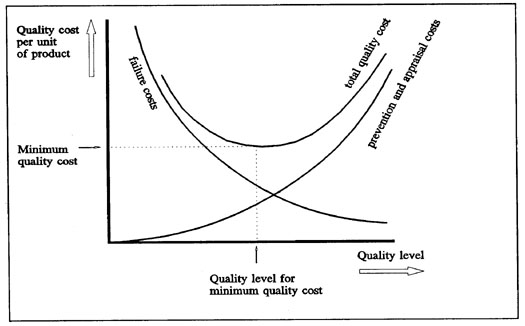
\includegraphics[width=\linewidth]{qm/swq-level}
\else
\begin{figure}[H]
\begin{center}
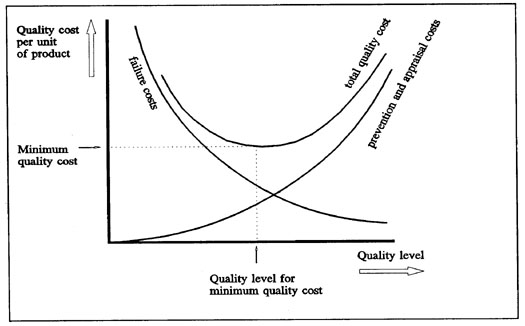
\includegraphics[width=\linewidth]{qm/swq-level}
\end{center}
\caption{SW-Quality Cost (Source
  \href{http://softwarequalityonline.blogspot.com/}
  {softwarequalityonline.blogspot.com/})}
\end{figure}
\fi
%\vspace{0.5cm}
%
\newpage
\section{Consequences}
Das Qualitätsmanagement muss umfassend sein: %das ganze Unternehmen erfassen:
% und f\"uhrt zwangsl\"aufig zu deren Umgestaltung.
\begin{itemize}
\item \structure{Verpflichtung zu ethischen Grundsätzen}
   (Beispiel siehe Anhang):
  Sicherheit, Gesundheit, Wohlergehen, Rücksichtnahme, Ehrlichkeit,
  Kritikfähigkeit, Fairness, Ver\-bes\-se\-rung und Weiterbildung
\item \structure{Respektierung der Mitarbeiter/-Innen}:
 mehr Selbstverantwortung,
 Vertrauen in die eigenen
 Erzeugnisse, erh\"ohte Motivation, geringere Arbeitsplatzfluktuationen\\
\end{itemize}
\ifslides
\newpage
\fi
%{\large\bf Grunds\"atze}
%\begin{itemize}
%\item Qualit\"at kann nicht im erpr\"uft -- sie muss vielmehr
%  erzeugt werden.
%\item Qualit\"atssicherung ist kein reiner Kostenfaktor sondern eine
%        Produktionsvoraussetzung.
%\item Grundlage bildet die Unternehmenskultur:
%\begin{itemize}
%       \item Ordnung und Systematik in der Organisation
%        \item Ehrlichkeit und Transparenz im Umgang mit den Mitarbeitern
%        \item Einsehen, dass man nicht perfekt ist.
%\end{itemize}
%\end{itemize}
%\subsection{Strategien}
%\begin{itemize}
%\item Defect Management Based Approach (Fehlerbekämpfung)
%
%A software defect can be regarded as any failure to address the end-user's
%requirements. Common defects include missed or misunderstood requirements and
%errors in design, functional logic, data relationships, process timing,
%validity checking, coding, etc.
%
%The defect management approach is based on counting and managing
%defects. Defects are commonly categorized by severity, and the numbers in each
%category are used for planning. More mature software development organizations
%use tools such as defect leakage matrices (for counting the numbers of defects
%that pass through development phases prior to detection) and control charts to
%measure and improve development process capability.
%
%\item Quality Attributes Approach
%
%This approach to software quality is best exemplified by fixed quality models,
%such as ISO/IEC 9126. This standard describes a hierarchy of six quality
%characteristics, each composed of sub-characteristics
%\end{itemize}
%
\section{Process}
Planen $\longrightarrow$ Lenken $\longrightarrow$ Bewerten $\longrightarrow$
Fördern
\begin{itemize}
\item \structure{Qualitätsplanung}: Festlegung der Qualitätsanforderungen
 und -ziele, sowie der zu verwendenden Methoden und Werkzeuge.
\item \structure{Qualitätslenkung}: Steuerung und Überwachung des
  Entwicklungsprozesses
  zur Sicherstellung, dass die Qualitätsziele erreicht werden,
  alle Arbeitstechniken und Tä\-tig\-kei\-ten, die zur Erfüllung der
  Qualitätsanforderungen angewendet werden. (ISO 8402)
\ifslides
\newpage
\fi
\item \structure{Qualitätsbewertung/-prüfung}: Durchführung von Massnahmen,
  die sicherstellen, dass die Produkt-
  und Prozessqualität den Anforderungen und Zielen entspricht.
  \begin{description}
  \item[Validierung] (validation) Feststellung, ob die spezifizierten
  Anforderungen an eine Komponenten oder ein System erfüllt sind.
  (Wird überhaupt das richtige Produkt entwickelt?)
\item[Verifikation] Feststellung, ob ein Arbeitsergebnis den für den
    betreffenden Arbeitsschritt gegebenen Vorgaben genügt.
    (Wird das Produkt richtig entwickelt?) Eventuell erfolgt dies durch
    mathematisch formale Beweisführung.
% Verification: Confirmation by examination and provision of objective
%    evidence that specified requirements have been fulfilled [ISO/IEC 12207,
%    Software life cycle processes]. In other words, verification ensures that
%    ``you built it right''.
%
%Validation: Confirmation by examination and provision of objective evidence
%    that the particular requirements for a specific intended use are fulfilled
%   [ISO/IEC 12207, Software life cycle processes.] In other words, validation
%    ensures that ``you built the right thing''.
%
  \end{description}
\item \structure{Qualitätsförderung}: Systematische Verwertung von Produkt- und
  Prozessdaten zur Ver\-bes\-serung des Qualitätssystems.
\end{itemize}
\newpage
%--------------------------------------------------------------------------
\section{Software Quality Criteria}
\ifslides
{\small
\begin{tabular}{p{4cm}p{4cm}l}\hline
\else
\vspace{1.5cm}

\begin{tabular}{p{5cm}p{5cm}l}\hline
\fi
                &                       & Vollst\"andigkeit\\
                & Effektivit\"at        & Korrektheit\\
                &                       & Bedienbarkeit \\ \cline{2-3}
                &                       & Speicherbedarf \\
                & Effizienz             & Laufzeit \\
                &                       & Interoperabilit\"at\\ \cline{2-3}
Benutzerakzeptanz &                     & Robustheit\\
                &                       & Sicherheit\\
                & Zuverl\"assigkeit     & Wiederherstellbarkeit\\
                &                       & Verf\"ugbarkeit \\
                &                       & Kontrollierbarkeit \\
                &                       & Pr\"ufbarkeit \\
\hline
\ifslides
\end{tabular}
}\newpage
{\small
\begin{tabular}{p{4cm}p{4cm}l}\hline
\fi
                &                       & Transparenz \\
                & Wartungsfreundlichkeit & Modularit\"at \\
                &                       & Normengerechtigkeit \\ \cline{2-3}
Ausbauf\"ahigkeit &                     & Portabilit\"at \\
                & Anpassungsf\"ahigkeit & Allgemeing\"ultigkeit \\
                &                       & Kopplungsf\"ahigkeit \\ \hline
\end{tabular}
\ifslides
}
\fi
\newpage
{\bfseries 6 Merkmale nach ISO 9126/25000:}
\ifslides
\begin{itemize}
\item \structure{Funktionalität} (Functionality)
\item \structure{Zuverlässigkeit} (Reliability)
\item \structure{Gebrauchstauglichkeit} (Usability)
\item \structure{Effizienz} (Efficiency)
\item \structure{Wartbarkeit} (Maintainability)
\item \structure{Übertragbarkeit} (Portability)
\end{itemize}
\newpage
\fi
\begin{description}
\item[Funktionalität] (Functionality) Vorhandensein von Funktionen mit
  festgelegten
  Eigenschaften, die die verlangten und impliziten Bedürfnisse abdecken
  \begin{itemize}
  \item Richtigkeit (Accurateness): die Funktionen liefern die richtigen oder
  vereinbarten
  Ergebnisse oder Wirkungen (Genauigkeit)
\item Angemessenheit (Suitability): Eignung der Funktionen für die verlangten
  Aufgaben.
\item Interoperabilität (Interoperability): Fähigkeit mit vorhandenen Systemen
  zu\-sam\-men zu wirken.
\item Ordnungsmässigkeit (Compliance): Erfüllung von anwendungsspezifischen
  Normen, Vereinbarungen, gesetzlichen Bestimmungen und ähnlichen
  Vorschriften.
\item Sicherheit (Security): Fähigkeit unberechtigten Zugriff, sowohl
  versehentlich als auch vorsätzlich auf Programme und Daten zu verhindern.
  \end{itemize}
\ifslides
\newpage
\fi
\item[Zuverlässigkeit] (Reliability) Fähigkeit der Software ihr
  Leistungs\-ni\-veau unter festgelegten Bedingungen über einen definierten
  Zeitraum zu bewahren.
  \begin{itemize}
  \item Reife (Maturity): geringe Versagenshäufigkeit durch Fehlzustände,
  geringe Stör\-an\-fäl\-lig\-keit.
  \item Fehlertoleranz (Fault tolerance): Fähigkeit, ein spezifiziertes
  Leistungs\-ni\-veau bei Software-Fehlern oder Nicht-Einhaltung ihrer
  spezifizierten Schnittstelle zu bewahren.
\item Wiederherstellbarkeit (Recoverability): Fähigkeit, bei einem Versagen
  das Leistungs\-ni\-veau wieder her zustellen und die direkt betroffenen Daten
  wieder zu gewinnen. Zu be\-rück\-sich\-tigen sind die dafür benötigte Zeit und der
  benötigte Aufwand.
  \end{itemize}
\ifslides
\newpage
\fi
\item[Gebrauchstauglichkeit] (Usability) Aufwand, der zur Benutzung
  erforderlich ist sowie die individuelle Beurteilung von festgelegten oder
  impliziten Benutzergruppen.
  \begin{itemize}
  \item Verständlichkeit (Understandability): Aufwand für den Benutzer, das
  Konzept und die Anwendung zu verstehen.
\item Erlernbarkeit (Learnability): Aufwand für den Benutzer
  die Bedienungsabläufe zu erlernen.
\item Bedienbarkeit (Operability): Aufwand für den Benutzer die Anwendung zu
  bedienen.
  \end{itemize}
\ifslides
\newpage
\fi
\item[Effizienz] (Efficiency) Verhältnis zwischen dem Leistungsniveau der
  Software und dem Umfang der eingesetzten Betriebsmittel unter festgelegten
  Bedingungen:
  \begin{itemize}
  \item Zeitverhalten (Time behaviour): Antwort- und Verarbeitungszeiten sowie
  Datendurchsatz bei der Funktionsausführung.
\item Verbrauchsverhalten (Resource behaviour): Anzahl der benötigten
  Betriebsmittel für die Erfüllung der Funktionen und Dauer der
  Betriebsmitteleinsatzes.
  \end{itemize}
\ifslides
\newpage
\fi
\item[Änderbarkeit] (Maintainability) Aufwand, der zur Durchführung
  vorgegebener Änderungen (Korrekturen, Verbesserungen, Anpassungen) notwendig
  ist.
  \begin{itemize}
  \item Analysierbarkeit (Analyzability): Aufwand um Mängel oder Ursachen von
  Stör\-un\-gen zu diagnostizieren oder um änderungsbedürftige Teile zu
  bestimmen.
\item Modifizierbarkeit (Changeability): Aufwand zur Ausführung von
  Verbesserungen, zur Fehlerbeseitigung oder Anpassung and
  Umgebungsänderungen.
\item Stabilität (Stability): Wahrscheinlichkeit des Auftretens unerwarteter
  Wirkungen von Änderungen.
\item Prüfbarkeit (Testability): Aufwand, der zur Prüfung der geänderten
  Software notwendig ist.
  \end{itemize}
\ifslides
\newpage
\fi
\item[Übertragbarkeit] (Portability) Eignung der Software von einer Umgebung
  in eine andere über\-tra\-gen zu werden. Umgebung kann organisatorische,
  Hardware- und Software-Um\-geb\-ungen einschliessen.
  \begin{itemize}
  \item Anpassbarkeit (Adaptability): Möglichkeit, die Software an an
  verschiedene, festgelegte Umgebungen anzupassen, wenn nur Schritte
  unternommen oder Mittel eingesetzt werden, die für diesen Zweck für die
  betrachtete Software vorgesehen sind.
  \item Installierbarkeit (Installability): Aufwand, der zum Installieren der
  Software in einer festgelegten Umgebung notwendig ist.
  \item Konformität (Conformance): Grad, in dem die Software Normen oder
  Verinbarungen zur Übertragbarkeit erfüllt.
  \item Austauschbarkeit (Replaceability): Möglichkeit die Software anstelle
  einer spezifizierten anderen in der Umgebung jener Software zu verwenden,
  sowie der dafür notwendige Aufwand.
  \end{itemize}
\end{description}
%--------------------------------------------------------------------------
%\section*{Qualit\"at und Qualit\"atssicherung.}
\section{Standards and Models}
\begin{tabular}{ll}\hline
{\bfseries ANSI / IEEE} & American National Standard Institute (www.ieee.org)\\
        &       Institute of Electrical and Electronics Engineers\\ \hline
%%& \\
 24765:2010 & Glossary of Software Engineering Terminology\\
 29119:2013 & Software Testing \\
 730-2014  & Software Quality Assurance Plans\\
  828-2012  & Software Configuration Management Plans\\
 829-2008  & Software Test Documentation \\
  29148:2011 & Software Requirement Specification \\
% Std 983-1986  & Software Quality Assurance Planning \\
  1008-1987 & Software Unit Testing \\
 1012-2012 & Software Verification and Validation Plans\\
% 1016-2009 & Software Design Description \\[2ex]
% Std 1028-2008 & Software Review and Audits
\ifslides
\end{tabular}
\newpage
\begin{tabular}{ll}\hline
\fi
{\bfseries ISO}     & International Standard Organisation  (www.iso.ch)\\ \hline
%%& \\
9000:2015 & Fundamentals and vocabulary / Grundlagen und Begriffe\\
9001:2015 & Requirements / Forderungen\\
9004:2009 & Guidance for performance improvement / Leistungsverbesserung\\
90003:2014 & Quality Management for Software Products and related
Services\\
9126  &  Qualitätskriterien für Software \\
15504     & Bewertung der Software-Entwicklungsprozesse\\
9241  & Ergonomic Requirements for Office Work with Visual Display
Terminals\\
14598 & Software Product Evaluation\\
15939 & Software Measurement Process\\
12119 & Quality Characteristics and Guidelines for their use \\
25000 & Software Product Quality Requirements and Evaluation (SQuaRE)\\
%\\[2ex] \hline
%{\bf SNV}       & Schweizerische Normenvereinigung (www.snv.ch)\\ \hline
%        & www.snv.ch, Postfach, 8032 Z\"urich \\[2ex] \hline
%{\bf SQS}       & Schweiz. Vereinigung f\"ur Qualit\"atssicherung, Bern\\ \hline
%        & befristete ISO-Zertifikate
\end{tabular}
\newpage
\ifslides
\begin{center}
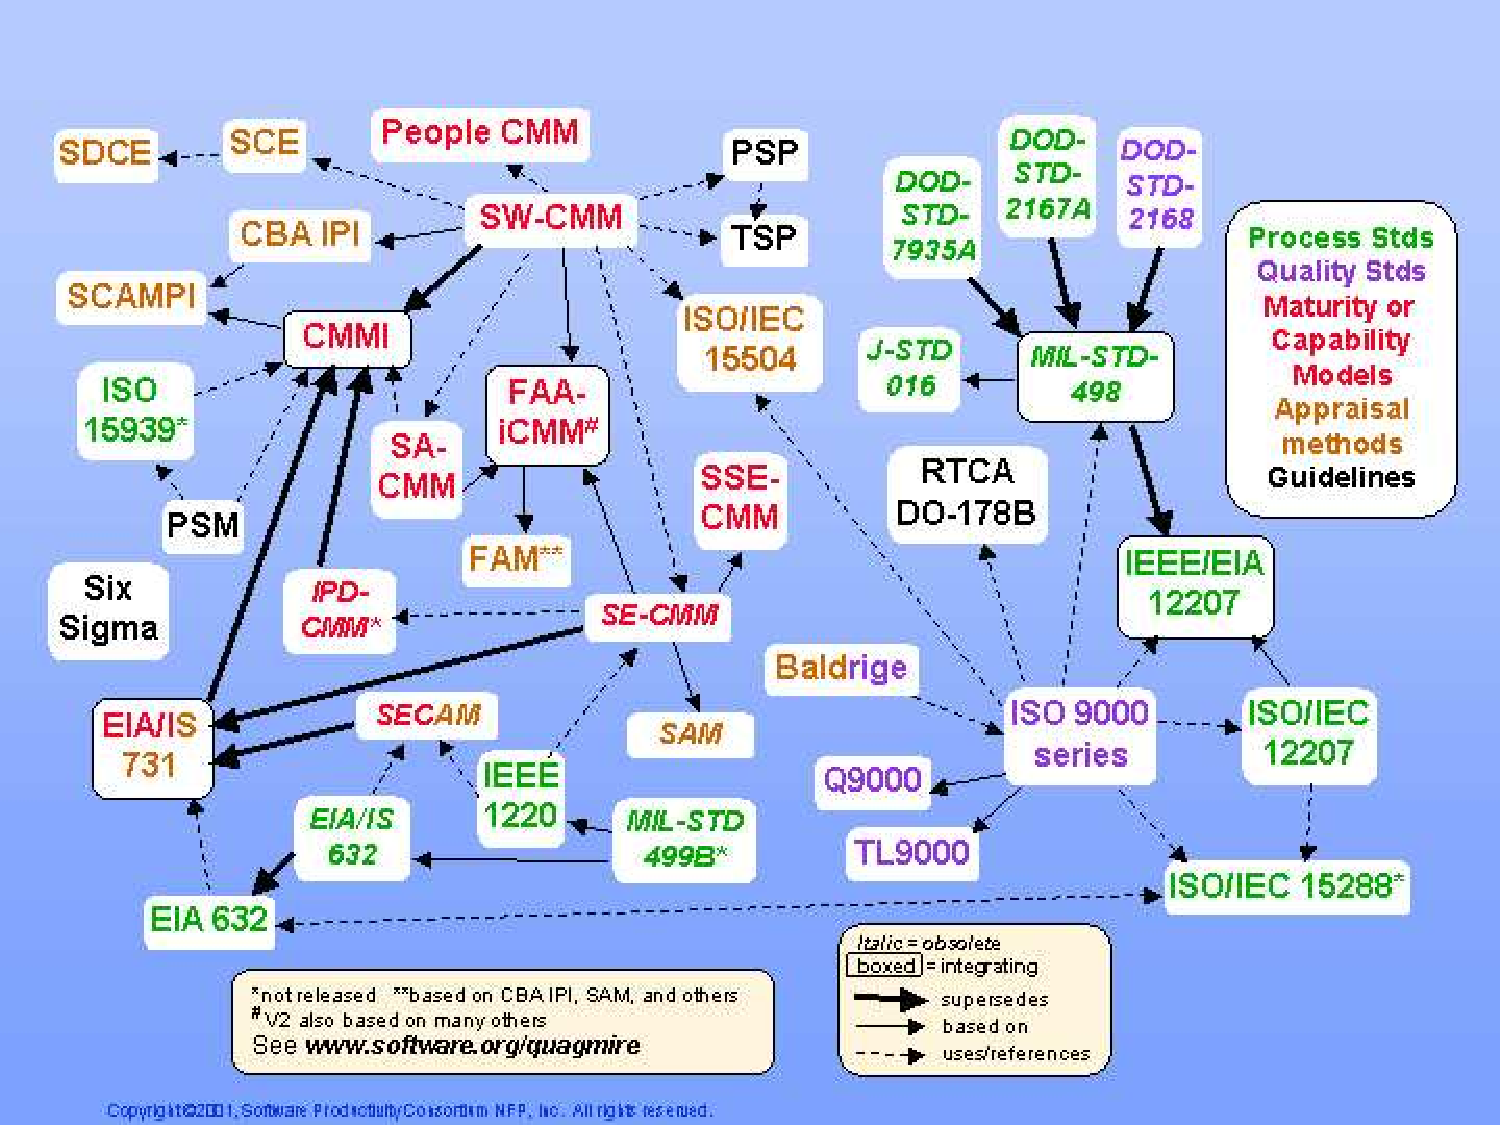
\includegraphics[width=0.85\linewidth]{qm/quagmap}
\end{center}
\newpage
\else
\subsection{A Quagmire of Standards?}
Im Softwareumfeld existieren zahlreiche Prozessstandards:

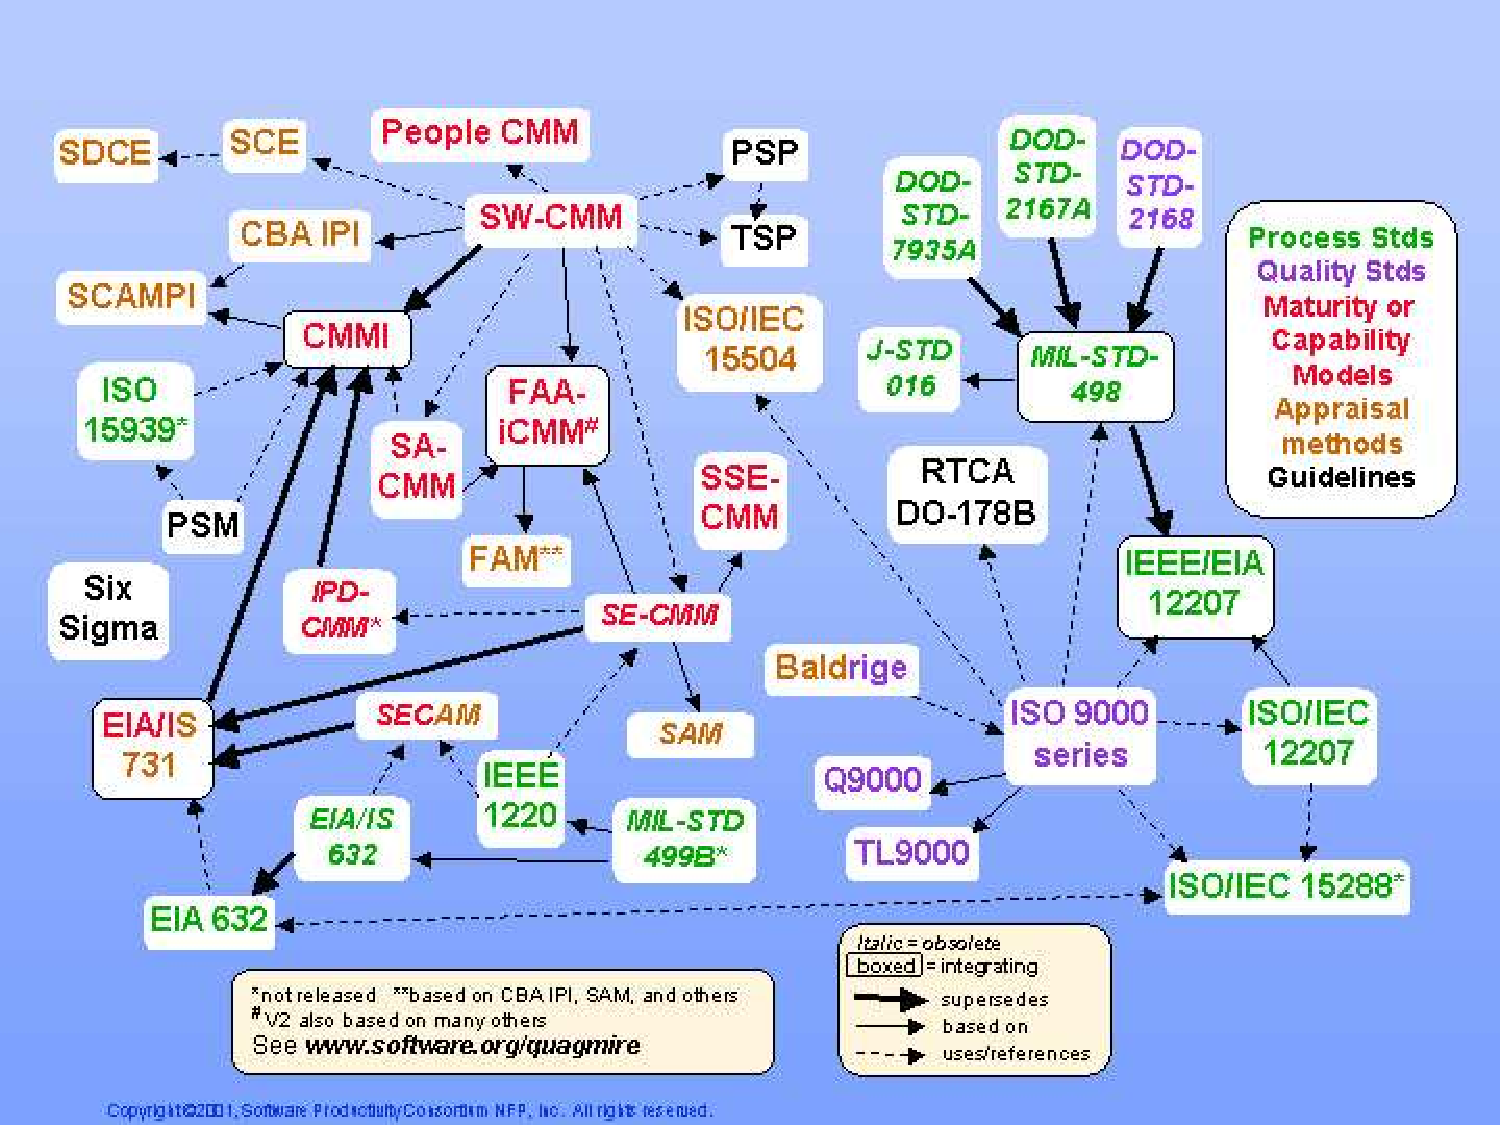
\includegraphics[width=\linewidth]{qm/quagmap}
\hfill Source: IEEE Computer July
2001 (S. 96-98)
\fi

%Organisationen:
%\begin{itemize}
%\item EIA: Electronics Industries Association
%\item DOD: Department of Defense
%\item \ldots
%\end{itemize}
\begin{itemize}
\item Process Standards enthalten Richtlinien für die
  Prozessgestaltung:
%
\begin{description}
\item [IEEE 1220:] Application and Management of the Systems
  Engineering Process, be\-schreibt die Tätigkeiten und Abläufe zur
  Entwicklung eines Systems
\item[ISO/IEC 12207:] Information Technology -- Software Life-Cycle Processes
  (1995)
  be\-schreibt den Rahmen eines Vorgehensmodells für die Erstellung und den
  Betrieb von SW-Produk\-ten, vom Konzept bis zur Ausserbetriebnahme. Das
  Modell
  umfasst die 5 primären Prozesse: Akquisition, Lieferung, Entwicklung,
  Unterhalt und Betrieb. Diese werden weiter unterteilt in Aktivitäten und
  Aufgaben (Tasks). Zudem werden 8 unterstützende Prozesse beschrieben:
  Dokumentation, Konfigurationsmanagement, Qualitätssicherung, Verifikation,
  Validation, Review, Audit und Problembehebung und die 4 organisatorischen
  Prozesse Management, Infrastruktur, Verbesserung und Schulung.
\newslide
\item[ISO/IEC 15288:] Systems Engineering -- System Life-Cycle Processes (2015)
  beschreibt den Rahmen eines Vorgehensmodells für die Erstellung und den
  Betrieb komplexer Systeme.
\item[ISO/IEC 15939:] Information Technology Software Engineering Software
  Measurement (2008): beschreibt einen flexiblen und anpassbaren Messprozess
  für die Software-Entwicklung und das System-Engineering.
\item[MIL-STD-498:] Software Development and Documentation (1994) einheitliche
  An\-for\-der\-ungen für die Softwareentwicklung und Dokumentation, spezifiziert
  Aktivitäten und Produkte, letztere in Detail in 22 ``Data Item Descriptions'' (DID)
\end{description}
%
\newslide
\item Quality Standards enthalten allgemeine Richtlinien zur Sicherstellung der
  Produkte- und Prozessqualität:
%
\begin{description}
\item [ISO 9000/9001:] beschreibt die Anforderungen an ein
  Qualitätsmanagementsystem
\end{description}
%
\newslide
\item Capability Models enthalten Richtlinien zur Verbesserung der
  Fähigkeiten einer Organisation:
%
\begin{description}
\item[SW-CMM:] Capability Maturity Model for Software (1993) ein fünfstufiges Modell zur
  Er\-höh\-ung des Reifegrades von Softwareprozessen.
\item[CMMI] Capability Maturity Model Integration (2001) ein einheitliches
  Modell zur Beurteilung der Entwicklungs- und Managementprozesse einer
  Organisation.
\end{description}
%
\newslide
\item Appraisal Methods enthalten Richtlinien zur Bewertung der
  Fähigkeiten von Organisationen:
%
\begin{description}
\item[ISO/IEC 15504:] Information Technology -- Software Process Assessment
  (2004) Durch\-füh\-rung von Assessments zur Fähigkeitsbestimmung und
  Prozess\-ver\-bes\-se\-rung
\end{description}
%
\item Guidelines enthalten Anweisungen für Arbeitsabläufe:
\begin{description}
\item[SixSigma] eine ursprünglich von Motorola
  entwickelte Methodik zur Prozess\-ver\-bes\-se\-rung durch Fehlerelimination
  basierend auf statistischen Analysen
\end{description}
\end{itemize}
\newpage
%--------------------------------------------------------------------------
\subsection{ISO 9000/9001/9004/90003}
Die ISO 9000 Normen wurden entwickelt um Unternehmen bei der Einführung
und dem Betrieb eines Qualitätsmanagements mit einem international
anerkannten, einheitlichen System effektiv zu unterstützen.
Die Unternehmen sollen damit Produkte erstellen kön\-nen,
die die Kundenforderungen und -erwartungen erfüllen und in
der Lage sein ihre Prozesse stetig
zu verbessern.

Um den Titel ``ISO 9001 zertifiziert'' zu verwenden, muss sich ein
Unternehmen von einer akkreditierten Stelle auditieren
lassen. Nach erfolgreichen Audits wird ein in der Regel
auf 3 Jahre befristetes
Zertifikat ausgestellt, welches nach Ablauf wieder erneuert werden kann.

\newslide
Grundsätze des Qualitätsmanagements:
\begin{enumerate}
\item {\bfseries Kundenorientierung:} Kundenerwartungen und -forderungen verstehen
  und erfüllen können,
\item {\bfseries Führung:} Schaffung eines Umfelds, in dem Menschen sich voll
 und ganz für die Unternehmensziele einsetzen können,
\item {\bfseries Einbeziehung der Personen:} Menschen sind das Wesentliche,
\item {\bfseries Prozessorientierter Ansatz:} zusammengehörige Mittel und
  Tätigkeiten als Einheit sehen,
\item {\bfseries Systemorientierter Managementansatz:} die Prozesse und ihre
  Wechselbeziehungen als System
  sehen, verstehen und lenken,
\item {\bfseries Kontinuierliche Verbesserung} als permanentes Ziel etablieren,
\item {\bfseries Sachbezogener Entscheidfindungsansatz:} effektive Entscheidungen
  basierend auf der logischen oder intuitiven Analyse von Daten und
  Informationen treffen,
\item {\bfseries Lieferantenbeziehungen zu gegenseitigem Nutzen}
\end{enumerate}
%
\begin{figure}[H]
\centering
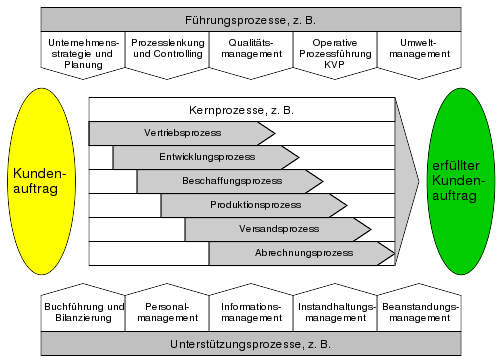
\includegraphics[width=0.66\linewidth]{qm/iso-prozess-orientierung}
\ifslides
\else
\caption{Prozessorientierung
     (Source: \href{http://www.iso9001.qmb.info}{www.iso9001.qmb.info})}
\label{fig:iso-prozess-orientierung}
\fi
\end{figure}
\begin{figure}[H]
\centering
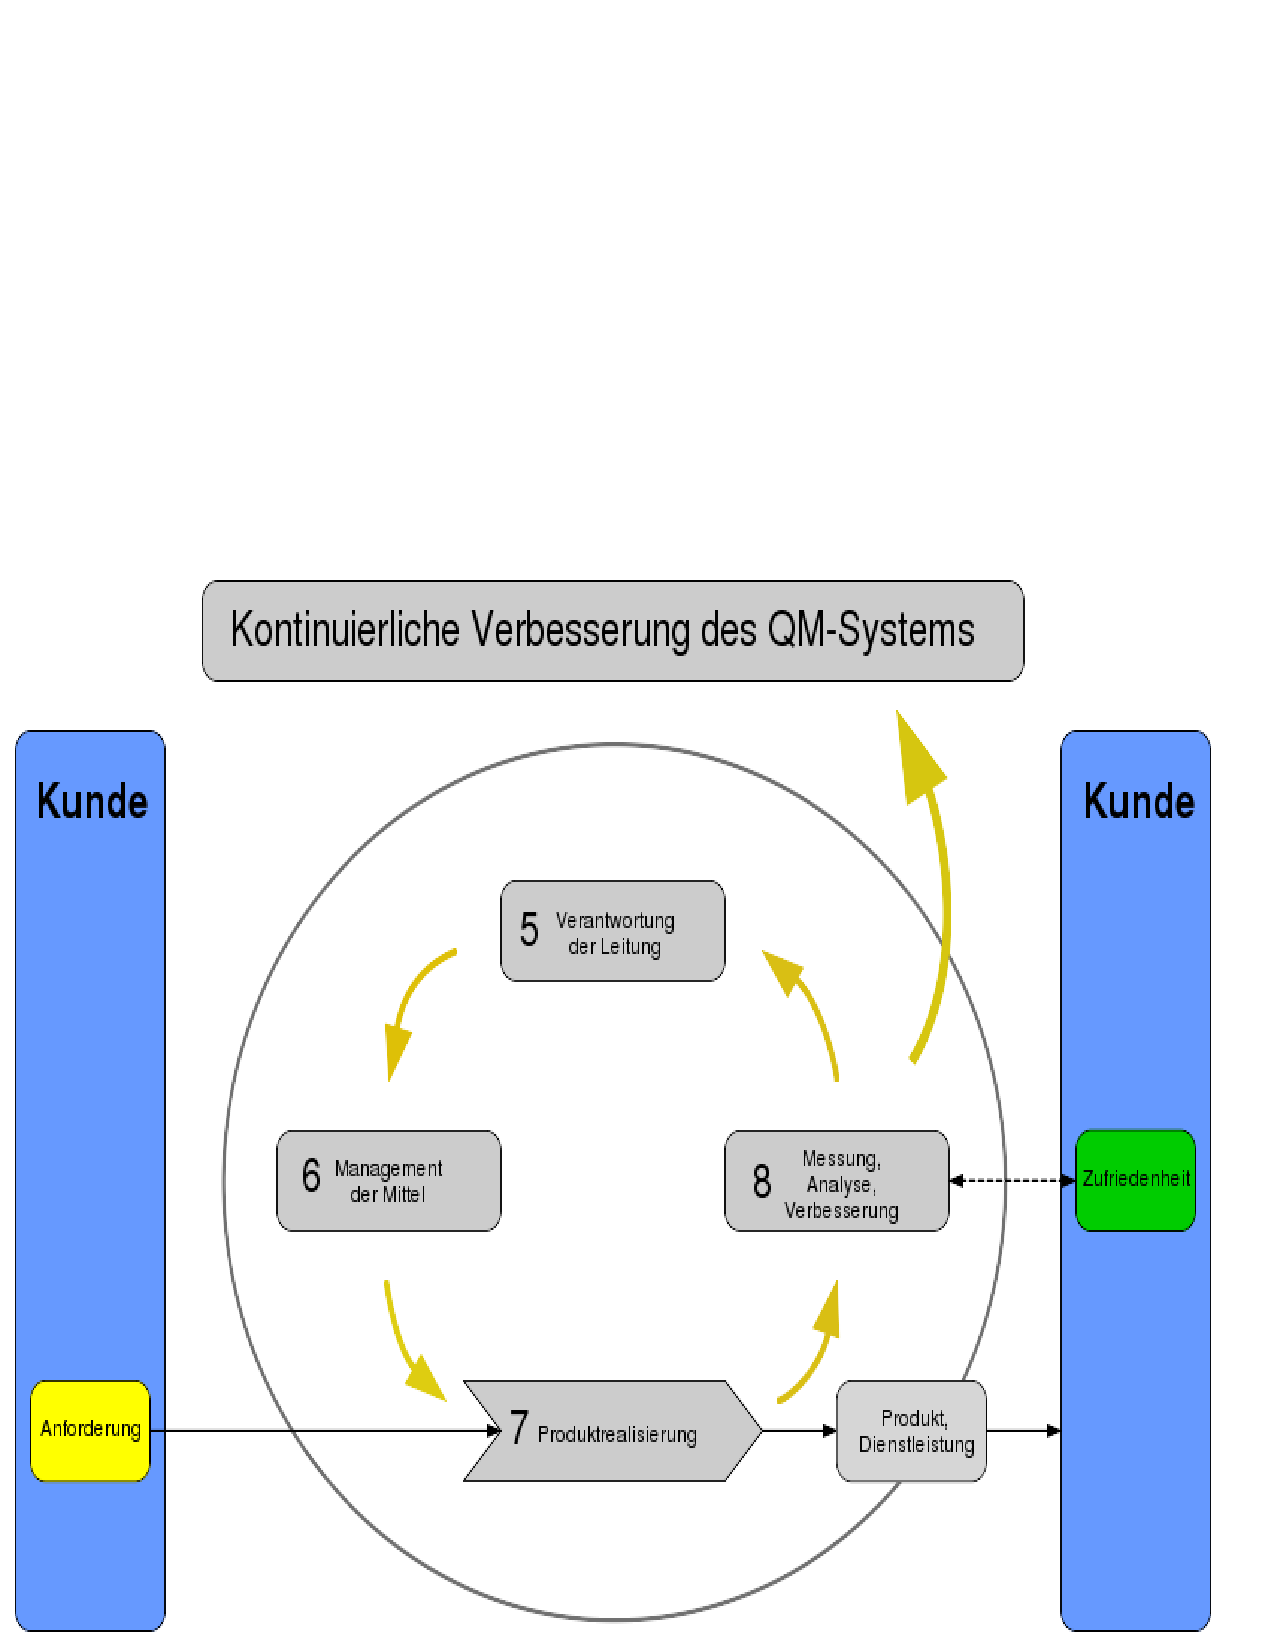
\includegraphics[width=0.66\linewidth]{qm/ISO}
\ifslides
\else
\caption{Modell eines prozess-orientierten QM-Systems
     (Source: \href{http://www.iso9001.qmb.info}{www.iso9001.qmb.info})}
\label{fig:iso}
\fi
\end{figure}
\ifslides
\newpage
\fi
Dokumentation: %kein Selbstzweck sondern wertsteigernde Tätigkeit
\begin{center}
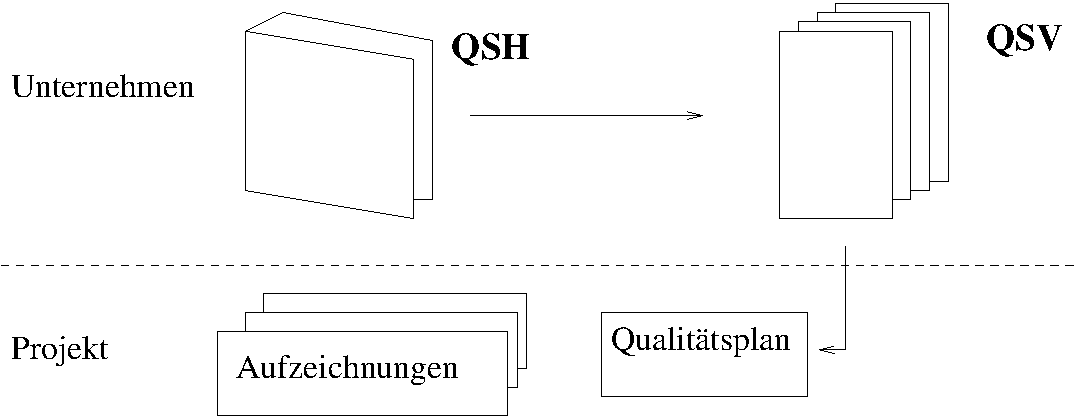
\includegraphics[width=0.7\linewidth]{qm/xfig/qsh-qsv}
\end{center}
\begin{description}
\item[Qualitätshandbuch:]  allgemeine Beschreibung des
  Qualitätsmanagementsystems nach innen und aussen
\item[QS-Verfahren:] Arbeitsanweisungen, Ablaufdiagramme und Formulare,
\item[QS-Plan:] Anwendung der QS auf ein bestimmtes Projekt,
\item[QS-Aufzeichnungen:] Nachweis über ausgeführte Tätigkeiten und Ergebnisse
\end{description}
\ifslides
\newpage
\fi
Mindestens die folgenden 6 Verfahren müssen dokumentiert sein:
\begin{itemize}
\item Lenkung der Dokumente (4.2.3)
\item Lenkung der Qualitätsaufzeichnungen (4.2.4)
\item Durchführung der internen Audits (8.2.2)
\item Lenkung fehlerhafter Produkte (8.3)
\item Korrekturmaßnahmen (8.5.2)
\item Vorbeugungsmaßnahmen (8.5.3)
\end{itemize}

Der auf 9001 basierende Standard 90003 enthält spezifische Anforderungen an das
Qua\-li\-täts\-manage\-ment von Software-Produkten und den damit zusammenhängenden
Dienst\-lei\-stungen für die Prozesse Beschaffung, Entwicklung, Betrieb, Unterhalt
und Zulieferung.

%Siehe \href{http://www.iso9001.qmb.info}{www.iso9001.qmb.info}
%
%--------------------------------------------------------------------------
%\newpage
\subsection{SEI-CMM Capability Maturity Model}
Das CM-Modell wird seit 1986 am Software Engineering Institute (SEI)
der Carnegie-Mellon Universität (Pittsburgh) im Auftrag der US-Regierung
entwickelt.

Ziel: Beurteilung von Software-Herstellern anhand einer Skala
 mit 5 Reifegraden\\[2ex]
\ifslides
{\small
\fi
\begin{tabular}{|ll|p{4.5cm}|p{4.5cm}|}
\hline
\multicolumn{2}{|l|}{Stufe}  & Charakteristiken & Notwendige Aktionen \\
\hline
1 & Initial & chaotisch, unzuverlässig, starke Streuung bei
                  Kosten, Terminen und Qualität
                         & Planung (Umfang, Kosten und Termine), Nachführung,
                           Konfigurationsmanagement, QS allg. \\
\hline
2 & Repeatable &  Schwankungen bei Kosten und Qualität,
                  angemessene Termintreue jedoch uneinheitliche Methoden
                  und Abläufe
                         & Prozess-Standards und Methoden für Analyse,
                            Design, Inspektionen und Prüfungen\\
\hline
3 & Defined &   gute Kosten- und Termintreue, verbesserte
               jedoch noch wechselnde Qualität
                         & Messungen, quantitative Qualitätsvorgaben  \\
\hline
4 & Managed &  zuverlässige und einheitliche Qualität der Produkte
                         &  quantitative Produktionspläne mit Nachführung
                            Prozessmessungen, Technologiemanagement\\
\hline
5 & Optimized & Basis für kontinuierliche Verbesserung von
             Produktivität und Qualität
                &  Konzentration auf fehlervorbeugende Massnahmen\\
\hline
\end{tabular}
\ifslides
}
\else
\newpage
\fi
\subsection{ISO 15504 / SPICE}
SPICE ({\bfseries S}oftware {\bfseries P}rocess {\bfseries I}mprovement
   \& {\bfseries C}apability d{\bfseries E}termination)
ist ein umfassender Standard zur Durchführung von Bewertungen
(Assessments) von Unternehmensprozessen mit Schwerpunkt auf der
Softwareentwicklung.
Das Referenzmodell von SPICE umfasst 48 Prozessbereiche (process
areas), die jeweils
bestimmte Ergebnisse (Outcomes) erzeugen und alle wichtigen Bereiche
einer Softwareentwicklungsorganisation abdecken.
\begin{figure}[H]
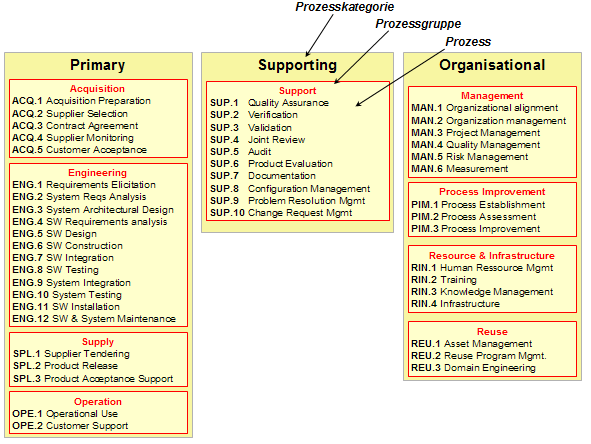
\includegraphics[width=\linewidth]{qm/Spice15504Processes}
\caption{Die Prozessgliederung des Referenzmodells}
\end{figure}

Die Prozessbereiche werden anhand von 9 Attributen
anlässlich eines Assessments
 einer Reifestufe zwischen 0 und 5
zugeordnet.

\begin{tabular}{|l|l|}
\hline
Reifestufe & Prozessattribute \\
\hline
5 Optimierend (Optimising) &   PA 5.1 Prozessinnovation\\
              &   PA 5.2 Prozessoptimierung\\
\hline
4 Vorhersagbar (Predictable) &  PA 4.1 Prozessmessung \\
               &  PA 4.2 Prozesssteuerung\\
\hline
3 Etabliert  (Established)  &  PA 3.1 Prozessdefinition \\
               &  PA 3.2 Prozessanwendung \\
\hline
2 Gemanagt   (Managed)  & PA 2.1 Managen der Prozessdurchführung\\
               & PA 2.2 Managen der Arbeitsprodukte \\
\hline
1 Durchgeführt (Performed) & PA 1.1 Prozessdurchführung\\
\hline
0 Unvollständig (Incomplete) & \\
\hline
\end{tabular}

\newslide
Die Bewertung der Prozessattribute erfolgt
aufgrund einer vierstufigen Skala:
\begin{description}
\item[N] (not achieved) nicht erfüllt
\item[P] (partially achieved) teilweise erfüllt
\item[L] (largely achieved) grösstenteils erfüllt
\item[F] (fully achieved) vollständig erfüllt
\end{description}

%Bewertung der Software-Entwicklungsprozesse:\\
%\begin{center}
%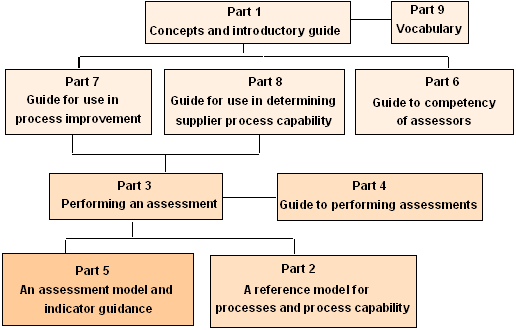
\includegraphics[width=0.9\linewidth]{qm/Spice15504Structure}
%\end{center}
%\begin{center}
%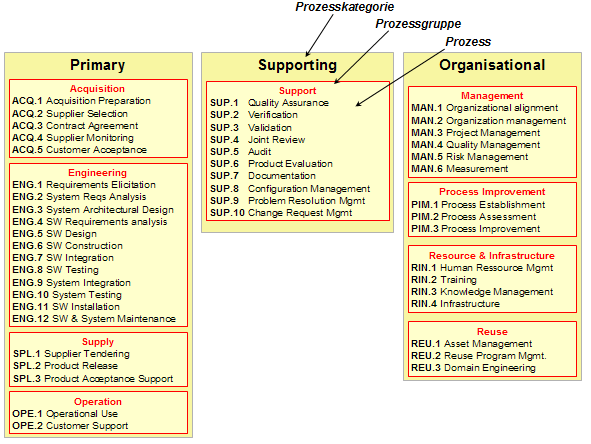
\includegraphics[width=0.9\linewidth]{qm/Spice15504Processes}
%\end{center}
%\begin{center}
%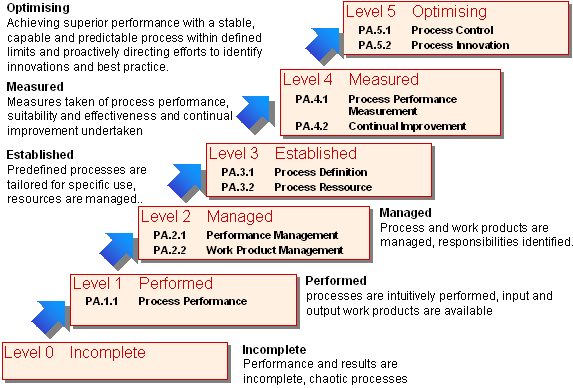
\includegraphics[width=0.9\linewidth]{qm/Spice15504Capability}
%\end{center}
\newpage
\subsection*{SPICE 1-2-1}
SPICE 1-2-1 (HM\&S GmbH)
\href{http://www.spice121.com}{www.spice121.com})
ist ein Werkzeug zur quantitativen
Analyse der relevanten Ge\-schäfts\-prozesse
eines Softwareunternehmens gem. ISO 15504.
%
%Es werden dabei 48 Prozessbereiche auf ihren Erfüllungsgrad anhand von
% 9 Kriterien untersucht:
\begin{figure}[H]
\begin{center}
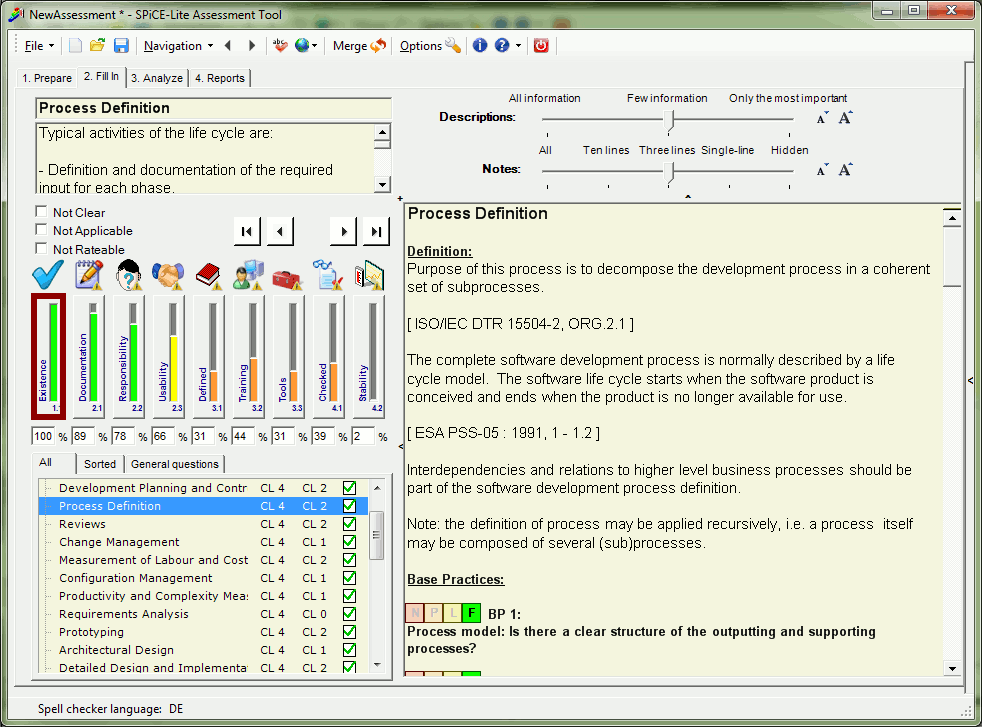
\includegraphics[width=0.75\linewidth]{qm/spice-prozesse}
\end{center}
\caption{Die Prozessbewertung mit Spicelite}
\end{figure}
%
%Nach durchgeführter Bewertung kann das Fähigkeitsprofil erstellt werden:
\begin{figure}[H]
\begin{center}
  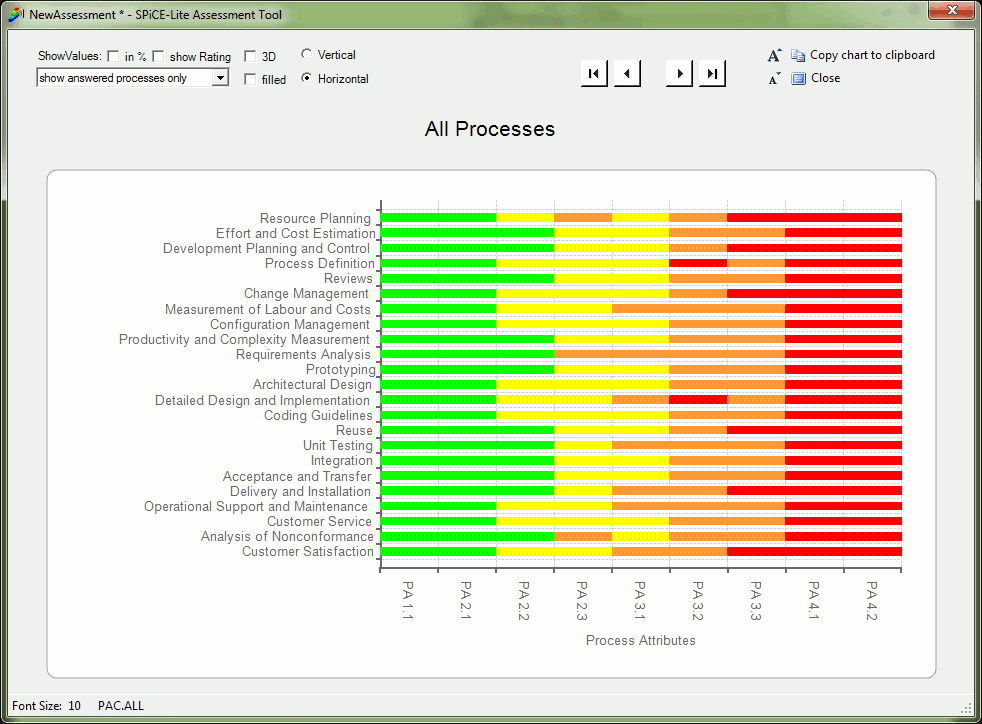
\includegraphics[width=0.75\linewidth]{qm/spice-bewertung}
\end{center}
\caption{Auswertung mit Spicelite}
\end{figure}
\newpage
%-------------------------------------------------------------------
\section{Quality Control and Assessment}
\ifslides
\else
%\vspace{1.5cm}
%
\begin{minipage}[t]{7cm}
\fi
\sloppy
vor und w\"ahrend der Fertigung\\[2ex]
{\bfseries Konstruktive Massnahmen}
\begin{itemize}
\item geeignete Prozessmodelle, Verfahren und Werkzeuge einsetzen
\item Qualit\"atsziele festlegen
\item Qualit\"atssicherungsplan erstellen:
        \begin{itemize}
        \item Programmier- und Dokumentationsrichtlinien
        \item Softwaretechniken
        \item Pr\"ufungen
        \item Verantwortlichkeiten
        \end{itemize}
\item Personalauswahl, Schulung
\end{itemize}
\ifslides
\newpage
\else
\end{minipage}
\hfill
\begin{minipage}[t]{7cm}
\sloppy
\fi
 nach der Fertigung \\[2ex]
{\bfseries Analytische Massnahmen}
                        \begin{itemize}
                        \item Begutachtung und Kontrolle
                                \begin{itemize}
                                \item Checklisten
                                \item Inspektionen / Walkthroughs
                                \item Autor-Kritikerzyklen
                                \item Review
                                \end{itemize}
                        \item Messungen und Tests
                        \item Bewertung
                        \item Veranlassung von Folgemassnahmen
                        \end{itemize}
\ifslides
\else
\end{minipage}
\fi

{\bfseries Ziel}: Minimierung des Aufwands für analytische Massnahmen durch
konsequente Anpassung, Verbesserung und Optimierung der konstruktiven
Massnahmen.
%------------------------------------------------------------------------
\ifslides
\newpage
\fi
\subsection{Quality Assurance Plan}
Die Beschreibung der projektspezifischen Massnahmen und Dokumente zur
Qualitäts\-si\-che\-rung:
(nach IEEE 730 Guide for Software Quality Assurance Planning)
%Kevin Daily Quality Management for Software)
\begin{enumerate}
\item Zweck {\em (Purpose)}\\
  die Bezeichnungen der Software-Komponenten, ihre beabsichtigten
  Einsatzbedingungen,
\item Referenzen {\em (Reference Documents)}\\
 das Projekt betreffende Qualitätssystemdokumente,
       Verträge, Standards, Richtlinien, Arbeitsanweisungen etc.
%\item Projektbeschreibung {\em (Project Description)}
\item Führung {\em (Management)}\\
Organisation, Verantwortlichkeiten, Aufgaben, Rollen, Ressourcen
\item Dokumentation {\em (Documentation)}\\
\ \ - Liste der zu erstellenden Dokumente: Anforderungsspezifikation,
Konfigurationsmanagementplan (SCMP), Software Verifikations- und
Validierungsplan (SVVP), Benutzeranleitung,
\ \ - Beschreibung der Review- und Kontrollprozeduren
\item Standards und Richtlinien {\em (Standards,
          practices, conventions and metrics )}\\
  die anzuwendenden Standards, Richtlinien und Verfahren und wie diese
          überwacht werden sollen.
\item Software Reviews {\em (Software Reviews)}\\
 Inspektionsaktivitäten und -techniken zur Kontrolle der Planeinhaltung
\item Test {\em (Test)}\\
   Liste der Tests, die nicht im SVVP enthalten sind.
 \item Problembehandlung und Nachbesserung {\em(Problem reporting and
 corrective action)}\\
 die Verfahren und Abläufe der Behandlung und Behebung von Störungen und
 Schwachstellen in den Software-Komponenten und Prozessen für Entwicklung und
 Unterhalt.
\item Methoden, Werkzeuge und Techniken {\em (Tools, techniques and
    methologies)}\\
   die anzuwendenden Werkzeuge, Methoden und Techniken.
%\item Code-Überwachung {\em (Code control)}\\
%   Bezeichnung der zu überwachenden Softwarekomponenten, Kennzeichnung,
%   Verzeichnisse, Backupmassnahmen, (ev. Referenzierung des SCMP)
 \item Ablage und Zugriffsregelungen {\em Media control)}\\
  Ablageinformation, Sicherheitskopien, Sicherstellung, dass nur authorisierte
  Personen Zugriff haben. (ev. Referenzierung des SCMP)
\item Dienstleistungen und Produkte Dritter {\em (Supplier Control)}\\
  Miteinbezug und Überwachung von Lieferanten und deren Produkte
\item Qualitätsaufzeichnungen {\em (Records collection, maintenance
    and retention)}\\
  die zu erstellenden Aufzeichnungen und ihre Archivierung zur
     Sicherstellung der Rück\-ver\-folg\-barkeit. (ev. Referenzierung des SCMP)
\item Ausbildung {\em (Training)}\\
   spezielle Ausbildungsmassnahmen.
%\item Fortschrittsüberwachung {\em (Progress Monitoring and Reporting)}
%\item Unterhalt {\em Maintenance}
\item Risikoüberwachung und -steuerung {\em (Risk management)}\\
  Die Methoden und Verfahren zur Aufdeckung, Überwachung und Steuerung der
  Projektrisiken.
\end{enumerate}
%
%% Web Content Accessibility Guidelines WCAG
%
\section{User-Interface Design Principles}
Die Normenreihe ISO 9241 beschreibt allgemeine Richtlinien zur Interaktion zwischen
Mensch und Computer mit dem Ziel gesundheitliche Schäden beim Arbeiten am
Bildschirm zu verhindern und dem Benutzer die Ausführung seiner Aufgaben zu
erleichtern. Ursprünglich bestand diese Reihe aus 17
Teilen. Mittlerweile (2006) wurde sie aktualisiert und durch einige
Teile ergänzt.
\newslide
Dabei wurde auch die Nummerierung angepasst:
\begin{itemize}
\item 1 Allgemeine Einführung
\item 2-11 Anforderungen: visuelle Anzeigen, Eingabegeräte,
  Farbdarstellungen etc.
\item 12 Informationsdarstellung
\item 13-17 Benutzerführung (Menüs, Kommandosprachen,
  Bildschirmformulare, etc,)
\item 110 (vorher 10) Grundsätze der Dialoggestaltung
\item 151 (neu) Leitlinien zur Gestaltung von Benutzungsschnittstellen für
  das World Wide Web
\item 171 (neu) Leitlinien für die Zugänglichkeit von Software
\item \ldots
\end{itemize}
\ifslides
\newpage
\fi
Im Teil 110 sind die folgenden Grundsätze für die ergonomische
Gestaltung und Bewertung von Software enthalten:
\ifslides
\begin{itemize}
\item \structure{Aufgabenangemessenheit} (Suitability for the task)
\item \structure{Selbstbeschreibungsfähigkeit} (Self-descriptiveness)
\item \structure{Steuerbarkeit} (Controllability)
\item \structure{Erwartungskonformität, Verlässlichkeit} (Conformity with user
  expectations)
\item \structure{Fehlerrobustheit} (Error tolerance)
\item \structure{Individualisierbarkeit}
\item \structure{Lernförderlichkeit}
\end{itemize}
\newpage
\fi
\begin{itemize}
\item \structure{Aufgabenangemessenheit} (Suitability for the task): Die
  Unterstützung der Arbeitsaufgabe ohne unnötige Belastung: kurze Ladezeiten,
  Ein- und Ausgabe relevanter Daten, Menu-Short-Cuts für häufige Funktionen,
  sinnvolle Grundeinstellungen.
\ifslides
\newpage
\fi
\item \structure{Selbstbeschreibungsfähigkeit} (Self-descriptiveness):
  verständliche Erläuterung des
  Einsatzzweckes, des Leistungsumfanges und der Dialogschritte auf
  Verlangen, Zustandsmitteilung bei länger dauernden Operationen
\ifslides
\newpage
\fi
\item \structure{Steuerbarkeit} (Controllability): Beeinflussung der
  Geschwindigkeit und Reihenfolge des Ablaufes, Auswahl der Arbeitsmittel und
  Art und Umfang der Ein- und Ausgaben (Rück\-nehm\-bar\-keit,
  Detaillierungswahl, Dialogunterbrechung), Vergrösserung umfangreicher
  Gra\-fiken, Sortiermöglichkeit bei Listen und Tabellen
\ifslides
\newpage
\fi
\item \structure{Erwartungskonformität, Verlässlichkeit} (Conformity with user
  expectations): Deckungsgleich mit den Erfahrungen der Benutzer aus gleichen
  oder ähnlichen Arbeitsabläufen, konsistente Begriffe und Layout, Einhaltung
  von Systemstandards, Bsp: mit der Tabulator-Taste wird der Cursor von einem
  Eingabefeld zum nächsten bewegt, Anzeige von Sanduhr/Fortschrittsbalken bei
  länger dauernden Vorgängen (ab 2 Sek.)
\ifslides
\newpage
\fi
\item \structure{Fehlerrobustheit} (Error tolerance): das beabsichtigte
  Arbeitsergebnis kann trotz erkennbar fehlerhaften Eingaben ohne oder mit
  minimalem Korrekturaufwand erreicht werden: all\-ge\-mein-verständliche
  Hinweise,  Korrekturvorschläge, keine undefinierten System\-zu\-stände,
  einfache Plausibilitätsprüfungen
\ifslides
\newpage
\fi
\item \structure{Individualisierbarkeit}: Anpassung an die spezifischen
  Erfordernisse der Arbeitsaufgabe und die individuellen Fähigkeiten und
  Vorlieben des Benutzers, Platzierung der Dialogfenster, Schrifttyp und
  -grösse
\ifslides
\newpage
\fi
\item \structure{Lernförderlichkeit}: Unterstützung des Benutzers beim
  Erlernen des Dialogsystems: Guided Tour, Test-Modus
\end{itemize}
\ifslides
\newpage
\fi
\subsection{Style Guides}
Style Guides als produkt- oder herstellerspezifische
Richtlinien sorgen für
Konsistenz bezüglich der Seiten- und Dialogstrukturen, der Navigation, der
Textgestaltung, der Formulierungen, der Farben, der Bedienabläufe etc.\\

\newslide
%\subsubsection*{Best Practices?}
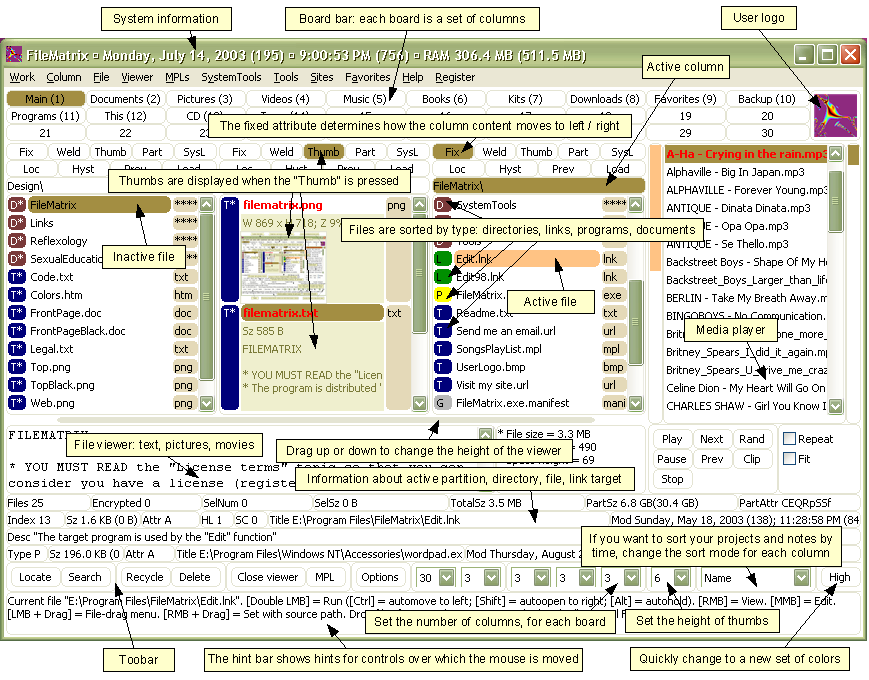
\includegraphics[width=\linewidth]{qm/o_filematrix}
% source http://destraynor.com/images/blog/o_filematrix.png

\newslide
Beispiele:
\begin{itemize}
\item Java Look and Feel Guidelines
\href{http://www.oracle.com/technetwork/java/jlf-135985.html}
    {www.oracle.com/technetwork/java/jlf-135985.html}
\item iOS Human Intercace Guidelines
  \href{https://developer.apple.com/ios/human-interface-guidelines/overview/design-principles/}{developer.apple.com}
\item Gnome Human Interface Guidelines
  \href{https://developer.gnome.org/hig/stable}
   {developer.gnome.org/devel/hig/stable}
 \item KDE Human Interface Guidelines \href{https://community.kde.org/KDE_Visual_Design_Group/HIG}
     {community.kde.org/KDE\_Visual\_Design\_Group/HIG}
   \item Windows User Experience Interaction Guidelines

     \href{https://developer.microsoft.com/en-us/windows/desktop/design}
          {developer.microsoft.com/en-us/windows/desktop/design}
%\href{http://msdn.microsoft.com/en-us/library/aa511258.aspx}
%   {msdn.microsoft.com/en-us/library/aa511258.aspx}
 \item Eclipse User Interface Guidelines
\href{http://wiki.eclipse.org/User_Interface_Guidelines}
   {wiki.eclipse.org/User\_Interface\_Guidelines}
% \item Java Swing Programming
%   \href{http://www.cs.cf.ac.uk/Dave/HCI/HCI_Handout_CALLER}
%         {www.cs.cf.ac.uk/Dave/HCI/HCI_Handout_CALLER}
%highly recommended!
%
\end{itemize}
\begin{figure}[H]
\ifslides
\centering
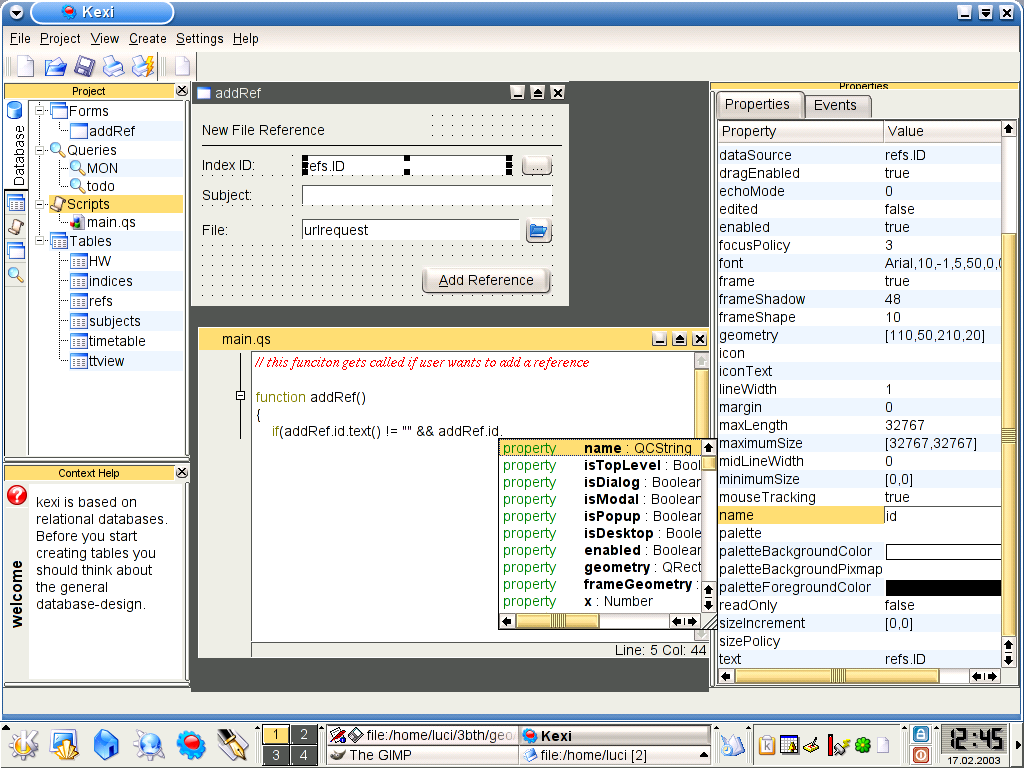
\includegraphics[width=0.9\linewidth]{qm/kexi-form-scripting}
\else
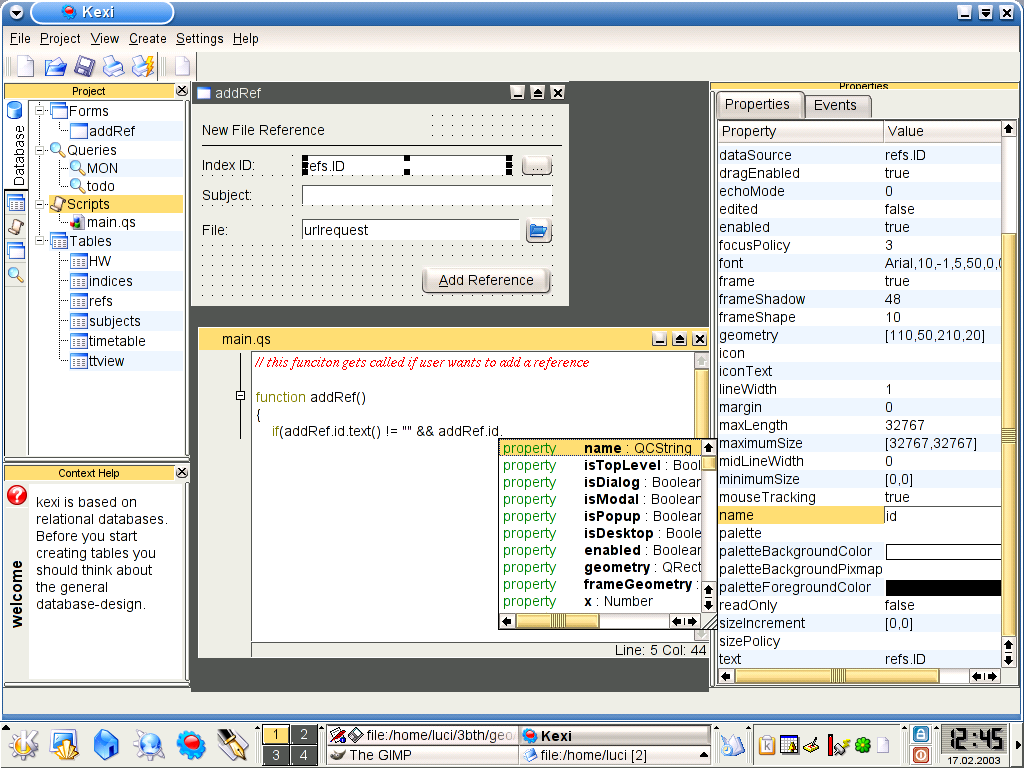
\includegraphics[width=\linewidth]{qm/kexi-form-scripting}
\fi
\caption{Kexi, an integrated data management application.}
\end{figure}
% http://stackoverflow.com/questions/2337323/gui-guidelines-for-swing
% http://www.miglayout.com/
%
\subsection{Java Look and Feel Design Guidelines}
The following is
a brief and rather incomplete summary of the Book ``Java Look and Feel Design
Guidelines'' (Second Edition) published by Sun Microsystems:

%The guidelines consist of 4 parts:
%\begin{enumerate}
%\item Overview: Java Look and Feel, Java Foundation Classes
%\item Fundamental Java Application Design: Application and Applets,
%  Accessibility, Internationalization, Themes, Layout, Text, Animation,
%  Colors, Icons, Mouse and Keyboard Operations, Drag-and-Drop
%\item The Components of the Java Foundation Classes: Windows, Panels, Scroll,
%  Tabbed and Split Panes, Dialogs, Menus and Toolbars, Buttons, Checkboxes,
%  Radio Buttons, List Boxes, Combo Boxes, Sliders, Labels, Text Fields,
%  Tables, Trees
%\item Backmatter: Short Cuts, Mnemonics, Navigation \ldots
%\end{enumerate}
\begin{enumerate}
\item \structure{Windows}

Graphical user interfaces are fundamentally based on windows.
A window is a user interface element and container that designers use to
organize the information that users see in an application. The information in
a window consists of objects (and their properties) that enable users to
perform actions or to report information about actions. Primary windows,
secondary windows, utility windows, and plain windows provide the top-level
containers for your application.
\newslide
\begin{enumerate}
\item A primary window is a window in which the
user's main interaction with the data or document takes place. An application
can use any number of primary windows, which can be opened, closed, minimized,
or resized independently.
\begin{figure}[H]
\centering
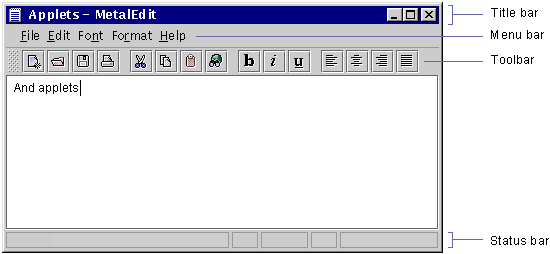
\includegraphics[width=0.9\linewidth]{qm/primary_window}
\caption{Elements of a primary window}
\end{figure}
\item A secondary window is a supportive window that is
dependent on a primary window (or another secondary window).
\item A utility window
is a window whose contents affect an active primary window. Unlike secondary
windows, utility windows remain open when primary windows are closed or
minimized. An example of a utility window is a tool palette that is used to
select a graphic tool.
\item A plain window is a window with no title bar or window
controls, typically used for splash screens.
\end{enumerate}
\newslide
\item \structure{Panels, panes and internal windows}

Panels, panes, and internal windows are lower-level containers for use
  within primary and secondary windows.
  \begin{enumerate}
  \item A panel is a container for organizing the contents of a window, dialog
    box, or applet.
  \item A pane is a collective term for scroll panes, split panes, and tabbed
    panes, which are described in this chapter. (You can place panels in panes
    or panes in panels.)
  \item An internal window is a container used in MDI applications to create
  windows that users cannot drag outside of the main backing window.
\newslide
\item Primary windows act as top-level containers for the user interface
  elements that appear inside them. A primary window might hold a series of
  embedded containers. For example, a primary window in your application could
  have this organization:
\begin{itemize}
\item The window frame contains a menu bar and a panel
\item The menu bar contains menus
\item The panel contains a toolbar and a scroll pane and scrollbar
\item The toolbar contains toolbar buttons
\item The scroll pane contains an editor pane with a plug-in editor kit for
  styled text
\end{itemize}
\newslide
\begin{figure}[H]
\centering
  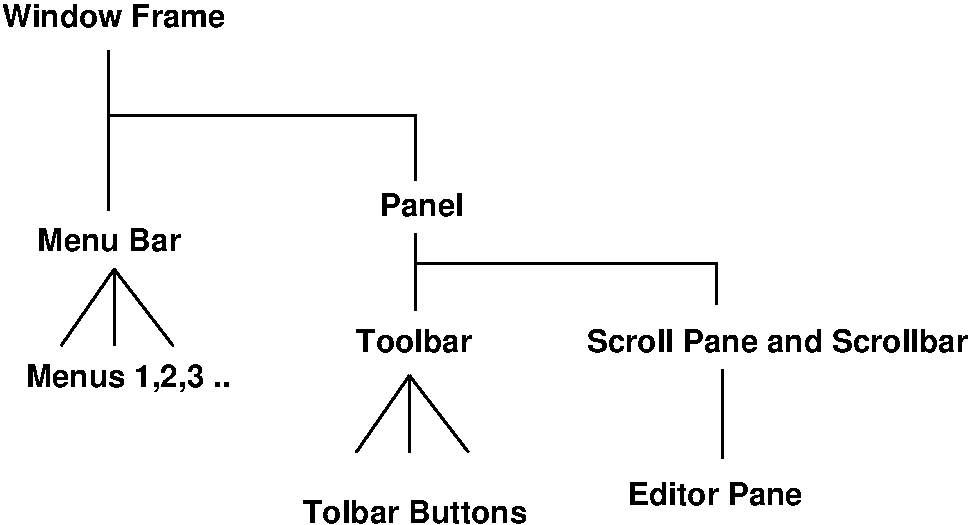
\includegraphics[width=0.8\linewidth]{qm/xfig/anatomy-of-a-window}
\ifslides
\else
  \caption{Components Contained in a Primary Window}
\fi
\end{figure}
\end{enumerate}
%
\newslide
\item \structure{Dialog boxes}
\begin{enumerate}
\item A dialog box is a secondary window in which users perform a task that is
  supplemental to the task in the primary window. For example, a dialog box
  might enable users to set preferences or choose a file from the hard disk. A
  dialog box can contain panes and panels, text, graphics, controls (such as
  checkboxes, radio buttons, or sliders), and one or more command
  buttons. Dialog boxes use the native window frame of the platform on which
  they are running (in both non-MDI and MDI applications).
\item An alert box is a secondary window that provides for brief interaction
  with users. Alert boxes present error messages, warn of potentially harmful
  actions, obtain a small amount of information from users, or display
  messages. The basic alert box has a symbol that identifies the type of the
  alert, a textual message, and one or more command buttons. The layout of
  these components is determined by the JFC.
\setcounter{saveenum}{\value{enumii}}
\end{enumerate}
\newslide
Dialog boxes can be modal or modeless. A modal dialog box prevents users from
interacting with the application until the dialog box is dismissed. However,
users can move a modal dialog box and interact with other applications while
the modal dialog box is open. This behavior is sometimes called
``application-modal.''
\begin{enumerate}
\setcounter{enumii}{\value{saveenum}}
\item A modeless dialog box does not prevent users from interacting with the
application they are in or with any other application. Users can go back and
forth between a modeless dialog box and other application windows.
\item Use modeless dialog boxes whenever possible. The order in which users
 perform
 tasks might vary, or users might want to check information in other windows
 before dismissing the dialog box. Users might also want to go back and forth
 between the dialog box and the primary window.
\item Use modal dialog boxes when interaction with the application cannot
 proceed
 while the dialog box is displayed. For example, a progress dialog box that
 appears while your application is loading its data might be a modal dialog
 box if users can do nothing useful during the loading process
%
\begin{figure}[H]
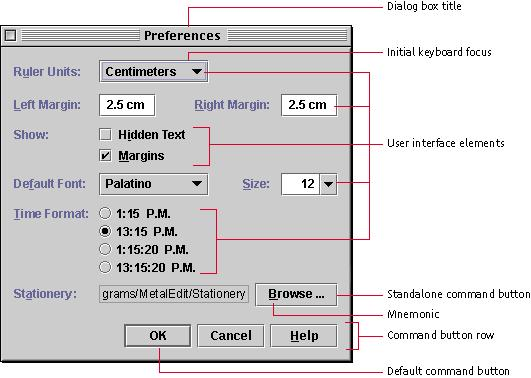
\includegraphics[width=\linewidth]{qm/java-dialog-std}
\ifslides
\else
\caption{Dialog Box Design.}
\fi
\end{figure}
%
\item In dialog boxes, include mnemonics for all user interface elements
  except the default button and the Cancel button.
\item When opening a dialog box, provide initial keyboard focus to the
  component that you expect users to operate first. This focus is especially
  important for users who must use a keyboard to navigate your application.
\item Consider the effect of internationalization on your design. Use a layout
  manager, which allows for text strings to become bigger or smaller when
  translated to another language.
\end{enumerate}
\newpage
\item \structure{Tab traversal order}
\begin{figure}[H]
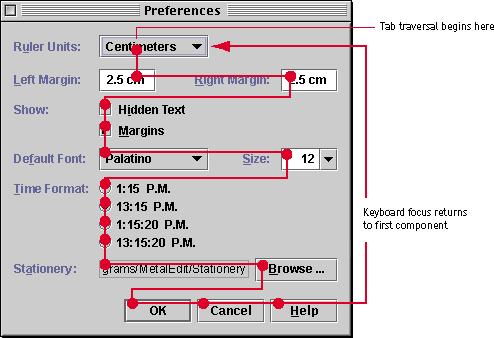
\includegraphics[width=\linewidth]{qm/java-dialog-stdTabTrav}
\ifslides
\else
\caption{Tab Traversal Order.}
\fi
\end{figure}
\begin{enumerate}
\item  Specify a logical tab traversal order for the user interface elements
  in a dialog box. The traversal order should match the reading order for your
  application's specified locale. For example, in English, the traversal order
  is left to right, top to bottom. By default, the traversal order is the
  sequence in which you added the components to the dialog box.
\item The setNextFocusableComponent method from JComponent can be used to
  specify the next component to receive keyboard focus. If a component is
  unavailable, it is skipped in the tab traversal order.
\end{enumerate}
\newpage
\item \structure{Menus}
\begin{figure}[H]
\centering
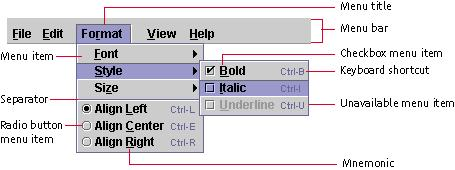
\includegraphics[width=0.7\linewidth]{qm/menus-MenuBar}
\caption{Pull-down Menu.}
\end{figure}
\begin{enumerate}
\item  Use a single word for each menu title.
\item Use menu titles that make it easy for users to determine which menu
  contains the items of interest to them. For example, the Format menu
  typically contains commands that enable users to change the formatting of
  their documents or data.
\item Be sure to include mnemonics for every menu title in your menu bar.
\item Do not display menu bars in secondary windows.
\item If you are writing an applet that runs in the user's current browser
  window (with the browser menu bar), do not display your own menu bar in the
  applet. Although applets displayed inside a browser window can have their
  own menu bars in the JFC, users are often confused when both the browser
  window and the applet have menu bars. If your applet requires a menu bar,
  display the applet in a separate browser window that does not have its own
  menu bar or navigation controls.
\item Even on Macintosh systems, which ordinarily place a menu bar only at the
  top of the screen, menu bars are displayed in windows for a Java look and
  feel application. On the Macintosh, the screen-top menu bar remains, but,
  since all the application menus are in the windows, the only command in the
  screen-top menu bar is Quit in the File menu. (Exit also appears in the File
  menu of primary windows.)
\end{enumerate}
\newpage
\item \structure{Tables and lists}
\begin{figure}[H]
\ifslides
\centering
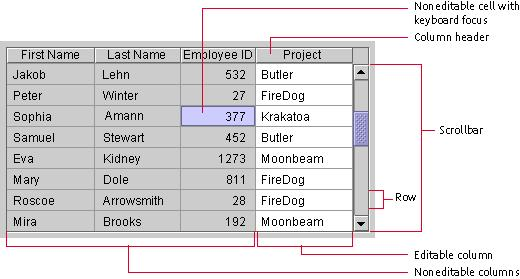
\includegraphics[width=0.95\linewidth]{qm/table-scell}
\else
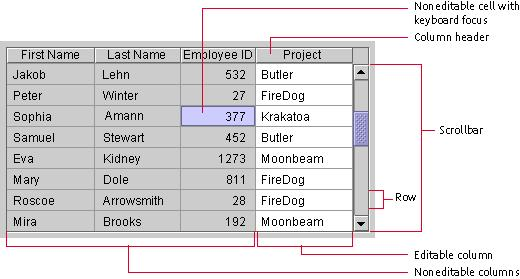
\includegraphics[width=\linewidth]{qm/table-scell}
\caption{Table in a Scroll Pane}
\fi
\end{figure}
\newslide
\begin{enumerate}
\item An unselected, editable cell gets its background color from the
  background of the table, which is white by default.
\item An unselected, uneditable cell gets its background from the secondary 3
  color which is gray in the default color scheme.
\item A selected, editable cell that has keyboard focus has a white background
  color. The inner border border is drawn in the primary 1 color to indicate
  that the cell has keyboard focus.
\item A selected cell that is noneditable and currently has keyboard focus
  gets its background color from the primary 3 color, which is light blue in
  the default color theme. The inner border is primary 1.
\item Any other selected cell gets its background color from the primary 3
  color, which is light blue in the default color theme.
\newslide
\item Selectable lists are appropriate when you want a user to select a few
  items
from a long list so that your application can then display details of the
selected items in a table. The user selects an item in the list on the left
(in left-to-right locales) and presses the Add button. The selected item is
removed from the list on the left and appears (with additional detail) in the
table on the right. The most recently moved item appears selected in the
table, as shown in the following figure.
\newslide
\begin{figure}[H]
\centering
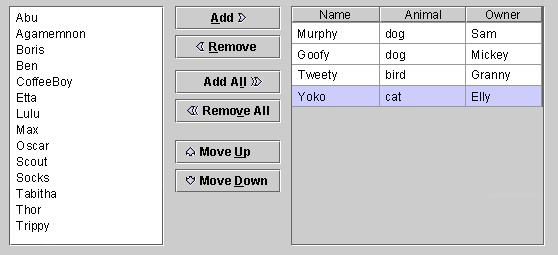
\includegraphics[width=0.8\linewidth]{qm/SelectableList1}
\caption{A Selectable List}
\end{figure}
\end{enumerate}
\end{enumerate}
%
% \item JavaToo:
%
\subsection{Auswahl des Java Look and Feel}
%
Das Look\&Feel von Java-Applikationen kann mit Hilfe
der Klasse UIManager zur Laufzeit festgelegt werden:
\begin{lstlisting}[language=java]
  UIManager.setLookAndFeel(
       "com.sun.java.swing.plaf.motif.MotifLookAndFeel" );
\end{lstlisting}
Die Web-Seite \href{http://www.javootoo.com}{www.javootoo.com}
bietet eine Sammlung freier und kostenpflichtiger
Look\&Feel-Bibliotheken.
\begin{figure}[H]
  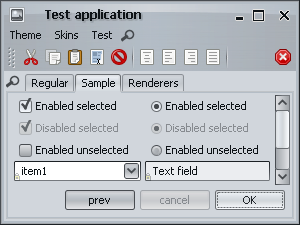
\includegraphics[width=0.25\linewidth]{qm/substancebusiness1}
\hfill
  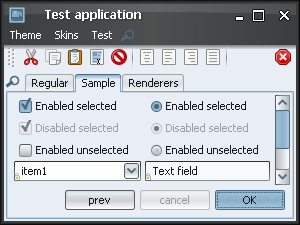
\includegraphics[width=0.25\linewidth]{qm/substancebusinessblacksteel1}
\hfill
  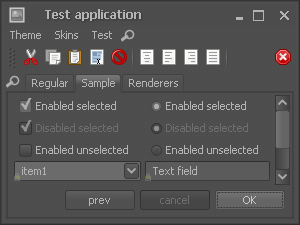
\includegraphics[width=0.25\linewidth]{qm/substanceravengraphite1}
  \caption{Substance Java Look\&Feel}
  \label{fig:substance}
\end{figure}

\subsection{Additional Examples}
\begin{minipage}{0.4\linewidth}
\begin{figure}[H]
\begin{center}
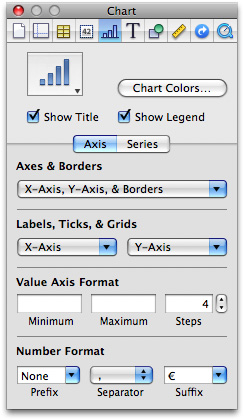
\includegraphics[width=\linewidth]{qm/apple_inspectorexample}
\caption{Ein OS-X-Dialog-Fenster}
\end{center}
\end{figure}
\end{minipage}
\hfill
\begin{minipage}{0.58\linewidth}
\begin{figure}[H]
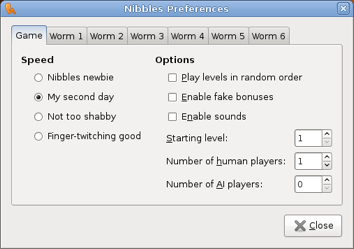
\includegraphics[width=\linewidth]{qm/gnome-preferences}
\caption{Ein Gnome Dialog-Fenster}
\end{figure}
\end{minipage}
\begin{figure}[H]
\begin{center}
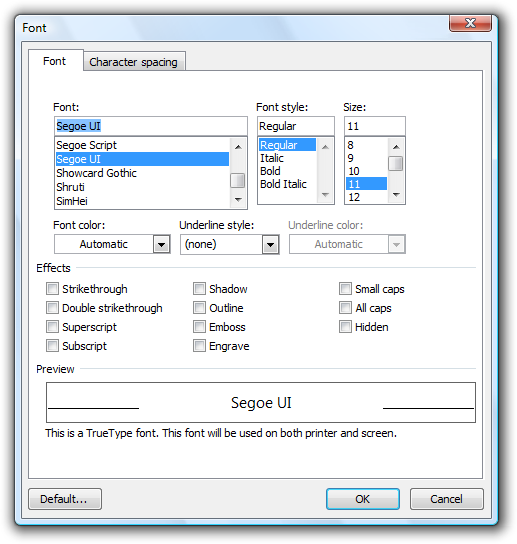
\includegraphics[width=0.45\linewidth]{qm/windows-dialog}
\caption{Ein Windows-Dialog-Fenster}
\end{center}
\end{figure}
%
% Label Placement in Forms
%  http://www.uxmatters.com/mt/archives/2006/07/label-placement-in-forms.php
%
\section{Code Conventions}
Programmierrichtlinien sorgen für einheitlichen Programmierstil und bessere
Lesbarkeit und senken dadurch den Wartungsaufwand, da fremder Code
schneller verstanden wird.

Kriterien:
\begin{itemize}
\item Conciseness (Prägnanz): einfache, klare, verständliche Anweisungen und
  Abläufe (Logik, Algorithmen),
\item Compliancy (Konformität): einheitliche Namenskonventionen für Variablen,
  Methoden, Klassen, Pakete, Anwendung etablierter Lösungsmuster,
\item Modularity (Modularität): gut strukturierte, gekapselte,
  d.h. entkoppelte Pakete, Klassen und Methoden
\end{itemize}

Beispiele
\begin{itemize}
\item Google \href{https://google.github.io/styleguide/javaguide.html}
            {google.github.io/styleguide/javaguide.html}
\item Sun \href{http://www.oracle.com/technetwork/java/index-135089.html}
          {www.oracle.com/technetwork/java/index-135089.html}
\end{itemize}
%\newcounter{saveenum}
%
\ifslides
\newpage
\fi
\begin{enumerate}
\setcounter{enumi}{2}
\item File Organization
  \begin{enumerate}
  \item Files longer than 2000 lines are cumbersome and should be avoided.
  \item Each Java source file contains a single public class or
  interface. When private classes and interfaces are associated with a public
  class, you can put them in the same source file as the public class. The
  public class should be the first class or interface in the file.
\item Java source files have the following ordering:
  \begin{itemize}
    \item Beginning comments %(see "Beginning Comments" on page 4)
    \item Package and Import statements
    \item Class and interface declarations
  \end{itemize}
\item The first component of a unique package name is always written in
  all-lowercase ASCII letters and should be one of the top-level domain names,
  currently com, edu, gov, mil, net, org, or one of the English two-letter
  codes identifying countries as specified in ISO Standard 3166, 1981.
  \end{enumerate}
\ifslides
\newpage
\fi
\setcounter{enumi}{5}
\item Declarations
  \begin{enumerate}
  \item One declaration per line is recommended since it encourages
  commenting. In other words,
    \begin{lstlisting}[language=java]
int level; // indentation level
int size;  // size of table
    \end{lstlisting}
    is preferred over
    \begin{lstlisting}[language=java]
int level, size;
    \end{lstlisting}
\ifslides
\newpage
\fi
  \item When coding Java classes and interfaces, the following formatting
  rules should be followed:
\begin{itemize}
    \item No space between a method name and the parenthesis ``(`` starting its
      parameter list
    \item Open brace ``\verb+{+'' appears at the end of the same line as the
        declaration statement
    \item Closing brace ``\verb+}+'' starts a line by itself indented to match
    its corresponding opening statement, except when it is a null statement
    the ``\verb+}+'' should appear immediately after the ``\verb+{+''
  \item Methods are separated by a blank line.
  \end{itemize}
\ifslides
\newpage
\fi
    \begin{lstlisting}[language=java]
class Sample extends Object {
    int ivar1;
    int ivar2;

    Sample(int i, int j) {
        ivar1 = i;
        ivar2 = j;
    }

    int emptyMethod() {}

    ...
}
    \end{lstlisting}
\ifslides
\newpage
\fi
\end{enumerate}
\setcounter{enumi}{9}
\item Naming Conventions
\begin{enumerate}
\item Class and Interface names should be nouns, in mixed case with the first
  letter of each
  internal word capitalized. Try to keep your class names simple and
  descriptive. Use whole words-avoid acronyms and abbreviations (unless the
  abbreviation is much more widely used than the long form, such as URL or
  HTML).
\item Methods should be verbs, in mixed case with the first letter lowercase,
  with the first letter of each internal word capitalized.
\ifslides
\newpage
\fi
\item  Except for variables, all instance, class, and class constants are in
  mixed case with a lowercase first letter. Internal words start with capital
  letters. Variable names should not start with underscore \_ or dollar sign \$
  characters, even though both are allowed.

  Variable names should be short yet meaningful. The choice of a variable name
  should be mnemonic- that is, designed to indicate to the casual observer the
  intent of its use. One-character variable names should be avoided except for
  temporary "throwaway" variables. Common names for temporary variables are i,
  j, k, m, and n for integers; c, d, and e for characters.
\item  The names of variables declared class constants and of ANSI constants
  should be all uppercase with words separated by underscores (``\_''). (ANSI
  constants should be avoided, for ease of debugging.)
\end{enumerate}
\ifslides
\newpage
\fi
\item Programming Practices
  \begin{enumerate}
  \item Don't make any instance or class variable public without good
  reason. Often, instance variables don't need to be explicitly set or
  gotten-often that happens as a side effect of method calls.

  One example of appropriate public instance variables is the case where the
  class is essentially a data structure, with no behavior. In other words, if
  you would have used a struct instead of a class (if Java supported struct),
  then it's appropriate to make the class's instance variables public.
\item It is generally a good idea to use parentheses liberally in expressions
  involving mixed operators to avoid operator precedence problems. Even if the
  operator precedence seems clear to you, it might not be to others-you
  shouldn't assume that other programmers know precedence as well as you do.
\begin{lstlisting}[language=java]
if (a == b && c == d)     // AVOID!
if ((a == b) && (c == d)) // RIGHT
\end{lstlisting}
  \end{enumerate}
\end{enumerate}
%
\section{Program Documentation}
Man unterscheidet in der Regel zwei Arten von Programmdokumentation:
\begin{description}
\item[API-Spezifikation:] Sie beschreibt die Schnittstelle (Application
  Programming Interface):
  Klassen, Vererbungsstrukturen, Methoden,
   Parameter, Randbedingungen, Wertebereiche  etc.
\item[Programmier-Handbuch:] (programming guide) Hier werden allgemeine
  Konzepte und Begriffe erörtert,
  die übergeordneten Zusammenhänge dargestellt und
  Anwendungsbeispiele beschrieben.
\end{description}
\newslide
Zur Erzeugung der Dokumentation direkt aus dem Quellkode
sind verschiedene Programme verfügbar, die
diese meist in mehrere Formate konvertieren können.
Zum Beispiel (ohne Anspruch auf Vollständigkeit):\\[2ex]
\begin{tabular}{lll}
Name  &  Formate & Homepage \\
Doxygen & HTML, RTF, \LaTeX & \href{http://www.doxygen.org}{www.doxygen.org}\\
Kdoc & HTML, man, \LaTeX & \href{http://sirtaj.net/projects/kdoc}{sirtaj.net/projects/kdoc}\\
Sphinx & HTML, \LaTeX, ePub & \href{http://www.sphinx-doc.org}{www.sphinx-doc.org}\\
%DOC++ & HTML, \LaTeX   & \href{http://docpp.sourceforge.net}{docpp.sourceforge.net} \\
%CCDOC & HTML    & \href{http://ccdoc.sourceforge.net}{ccdoc.sourceforge.net} \\
\end{tabular}

\newslide
Sie orientieren sich alle
an dem ebenso gut dokumentierten wie einfachen Format von
Javadoc\footnote{\href{http://www.oracle.com/technetwork/articles/java/index-137868.html}
     {www.oracle.com/technetwork/articles/java/index-137868.html}}
%\ifslides
%\newpage
%\fi
Ein Kommentar, der in die Dokumentation übernommen werden soll,
beginnt mit den drei Zeichen \verb+/**+ andere Kommentare
  werden ignoriert:
\begin{lstlisting}[language=java]
/** The String class represents a sequence of characters
 */
public class Sstring {
...
\end{lstlisting}
\newslide
Die so markierten Kommentare können mit Schlüsselwörtern ergänzt werden.
Zum Beispiel:\\[2ex]
\begin{tabular}{ll}
\verb+@author [eine Zeile Text]+ & Autor der Klasse \\
\verb+@version [eine Zeile Text]+ & Version (üblicherweise die \\
                                  & CVS-Variable \verb+$Id$+)\\
\verb+@see [eine od. mehrere Referenzen]+ & Klassen- od. Methoden-Referenzen  \\
\verb+@return [eine Zeile]+ & Beschreibung des Rückgabewertes \\
\verb+@exception [Liste mit Ausnahmen]+ & Exceptions \\
\verb+@param [...]+ & Beschreibung des Parameters \\
\end{tabular}
%\ifslides
%\newpage
%\fi
\newslide
\subsection{Rules and Recommendation}
\begin{enumerate}
\item Die Klassen und Methoden sollen in englischer Sprache dokumentiert werden.
\item Die Beschreibung einer Klasse oder Methode erfolgt vor ihrer Deklaration.
\item Die Beschreibung einer Methode beginnt mit einem Verb:
\begin{lstlisting}[language=java]
/** Converts all of the characters in this String
  * to lower case
  * @return the string converted to lower case
  */
  public Sstring toLower(){
  ...
  }
\end{lstlisting}
\item Jeder Parameter einer Methode soll mit \verb|@param| beschrieben werden,
 auch wenn seine Bedeutung offensichtlich ist.
\item Jeder Rückgabewert einer Methode soll mit \verb|@return| beschrieben
  werden.
\begin{lstlisting}[language=java]
/** Concatenates the specified string to the end of this
  * string.
  * @param str - the String that is concatenated to the
  *      end of this String.
  * @return a string that represents the concatenation of
  *   this object's characters followed by the string
  *   argument's characters
  */
   public Sstring concat(Sstring str){
   ...
   }
\end{lstlisting}
\end{enumerate}
%%
\newslide
\subsection{Doxygen Example}
\begin{figure}[H]
\begin{center}
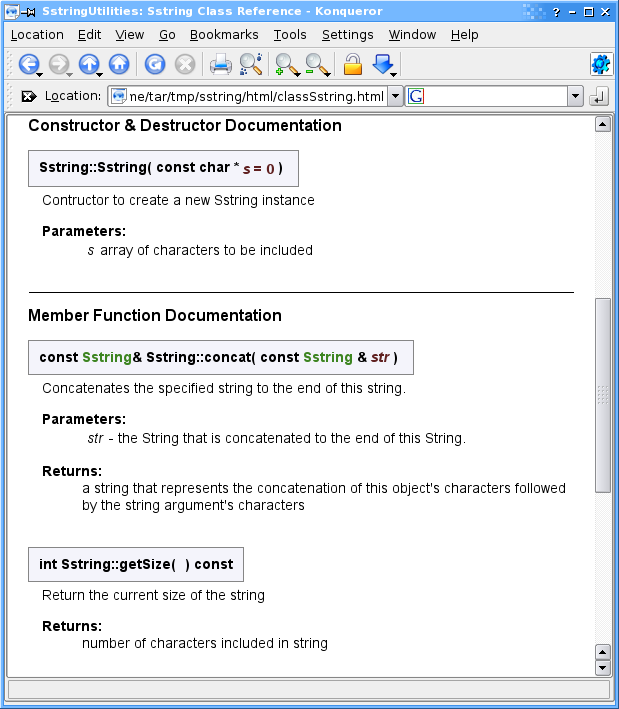
\includegraphics[width=0.6\linewidth]{qm/doxygen-example}
\end{center}
\caption{Mit Doxygen erzeugte Dokumentation in HTML-Format}
\end{figure}
Die folgenden Schritte sollen am Beispiel von Doxygen exemplarisch
zeigen, wie mit solchen Dokumentations-Generatoren gearbeitet
werden kann:
\begin{enumerate}
\item Man kreiert eine Konfigurationsdatei. Mit Hilfe dieser
  Datei kann die Erzeugung der
  Dokumentation gesteuert werden. Jedes Projekt sollte eine
  eigene Konfiguration besitzen, wobei ein Projekt aus einer
  einzelnen Datei oder aus mehreren unter einem Verzeichnisbaum
  abgelegten Dateien bestehen kann.

  Um die Erzeugung einer solchen Konfiguration zu vereinfachen,
  kann man mit
\begin{verbatim}
 doxygen -g <config-file>
\end{verbatim}
sich eine Vorlage erstellen lassen.

In der Konfigurationsdatei werden vorgegebenen Variablen bestimmte,
projektspezifische Werte zugewiesen:
\begin{verbatim}
TAGNAME = VALUE or
TAGNAME = VALUE1 VALUE2 ...
\end{verbatim}
Mit Ausnahme der Variable INPUT, begnügt man sich meist
mit den voreingestellten Werten. Die Variable INPUT
muss die Namen aller bei der Erzeugung der Dokumentation
zu berücksichtigten Dateien enthalten. Bei grösseren
Projekten weist man ihr lediglich die Namen der Verzeichnisse
zu und setzt die Variable FILE\_PATTERNS
zum Beispiel:
\begin{verbatim}
INPUT=src
FILE_PATTERNS=*.h
RECURSIVE=YES
\end{verbatim}
Hiermit werden alle im Verzeichnis \verb+src+ und darunter
liegenden Dateien, deren Name die Endung \verb+.h+
aufweist, berücksichtigt.
\item Erzeugung der Dokumentation:
\begin{verbatim}
 doxygen <config-file>
\end{verbatim}
Ohne entsprechende Anpassungen im Konfigurationsfile erzeugt
dieser Befehl im aktuellen Verzeichnis die Unterverzeichnisse
\verb|latex, rtf, html, man| an und füllt diese mit
den Dateien im jeweiligen Format.
\end{enumerate}
\begin{figure}[H]
\begin{center}
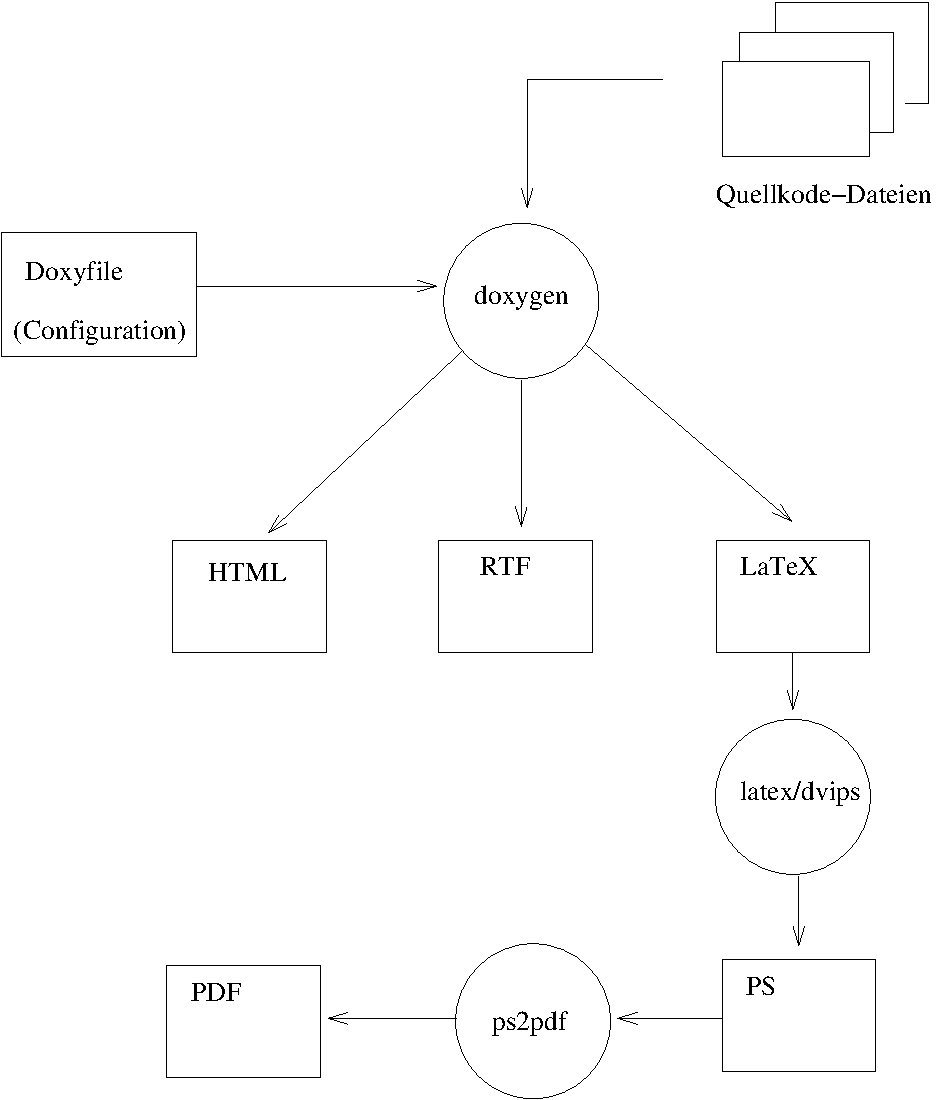
\includegraphics[width=0.9\linewidth]{qm/xfig/doxygen}
\caption{Ablauf der Dokumentgenerierung mit Doxygen}
\end{center}
\end{figure}
% \fi
%%%
%\newpage
\subsection{Javadoc Example}
Mit Javadoc, dem im Java-Standardpaket SDK enthaltenen
Dokumentationsgenerator, kann eine Dokumentation aus den mit public oder
protected bezeichneten Java-Klassen, Interfaces, Konstruktoren, Methoden und
Member-Variablen erzeugt werden. Die Dokumentation wird mit sogenannten {\em
  Doclets} erzeugt, das sind selbstdefinierbare Klassen, die die API des
Paketes com.sun.javadoc verwenden. Auf diese Weise kann das Ausgabeformat den
eigenen Bedürfnissen angepasst werden. Das Standard-Doclet erzeugt eine HTML-Dokumentation.

Beim Aufruf gibt man einen Paketnamen oder die Namen von Java-Dateien, deren
Dokumentation erzeugt werden soll:
\begin{verbatim}
javadoc [options] [packagenames] [sourcefilenames]
\end{verbatim}
\newslide
Javadoc bietet eine Vielzahl von Optionen. Zum Beispiel:

\begin{tabularx}{\linewidth}{lX}
\verb+-sourcepath <path-list>+ & Verzeichnisse in welchen Java-Dateien gesucht
                        werden\\
\verb+-classpath <classpath>+ & Verzeichnisse in welchen referenzierte Java-Klassen gesucht werden\\
\verb+-d <directory>+ & Verzeichnis, wo die Dokumentation abgelegt wird\\
\verb+-windowtitle <text>+   & Browser Window-Titel\\
\verb+-doctitle <html-code>+ & Titel der Übersichts-Seite (Overview)\\
\verb+-header <html-code>+   & Kopfzeile\\
\verb+-bottom <html-code>+   & Fusszeile\\
\end{tabularx}
\newslide
Die folgende Anweisung erzeugt eine HTML-Dokumentation aller Klassen des Pakets
ch.fhbb, die im Verzeichnis src gefunden werden, und legt die Dateien ins
Verzeichnis doc/html ab:
\begin{lstlisting}[language=csh]
% javadoc -d doc/html -sourcepath src ch.fhbb
\end{lstlisting}
\newslide
Man kann auch eine Datei erstellen, die die Javadoc-Argumente zeilenweise
auflistet:
\begin{verbatim}
-d doc/html
-sourcepath src
-windowtitle 'Scribble v1.4 API Specification'
-doctitle '<b>Scribble<b><br>v1.4'
-bottom 'Copyright 2009 FHNW. All Rights Reserved'
ch.fhnw
\end{verbatim}
Wenn man dieser Datei den Namen ``options'' zuweist, lautet der Aufruf:
\begin{lstlisting}[language=csh]
% javadoc @options
\end{lstlisting}
\newslide
Einfacher ist es jedoch, man verwendet Ant:
\begin{lstlisting}[language=xml
  ,morekeywords={target,mkdir,javadoc,packageset,doctitle,bottom}]
<target name="doc" >
  <mkdir dir="docs/api"/>
  <javadoc destdir="docs/api"
           author="true" version="true"  use="true"
           windowtitle="Test API" >
    <packageset dir="src" defaultexcludes="yes" />
    <doctitle> <![CDATA[<h1>For demo purposes only</h1>]]></doctitle>
    <bottom><![CDATA[
      <i>Copyright &#169; 2009 Dummy Corp. All Rights Reserved.</i>]]>
    </bottom>
  </javadoc>
</target>
\end{lstlisting}
\newslide
Noch besser eignet sich Maven:
\begin{lstlisting}[language=xml,
  morekeywords={reporting,plugins,plugin,artifactId,configuration,doctitle,bottom}]
<reporting>
  <plugins>
    <plugin>
      <artifactId>maven-javadoc-plugin</artifactId>
      <configuration>
        <doctitle> <![CDATA[<h1>For demo purposes only</h1>]]></doctitle>
        <bottom><![CDATA[
          <i>Copyright &#169; 2009 Dummy Corp. All Rights Reserved.</i>]]>
        </bottom>
      </configuration>
    </plugin>
</reporting>
\end{lstlisting}
\newslide
In Eclipse muss das Projekt im ``Package Explorer'' selektiert
werden. Anschliessend aktiviert man das File-Menu oder aktiviert mit der
rechten Maustaste das Popup-Menu und wählt ``Export''. Aus der angezeigten
Liste selektiert man javadoc. Mit ``Next'' erhält man die Möglichkeit noch
verschiedene Einstellungen zu definieren. Die eigentliche Erstellung wird mit
``Finish'' gestartet.
\begin{figure}[H]
  \centering
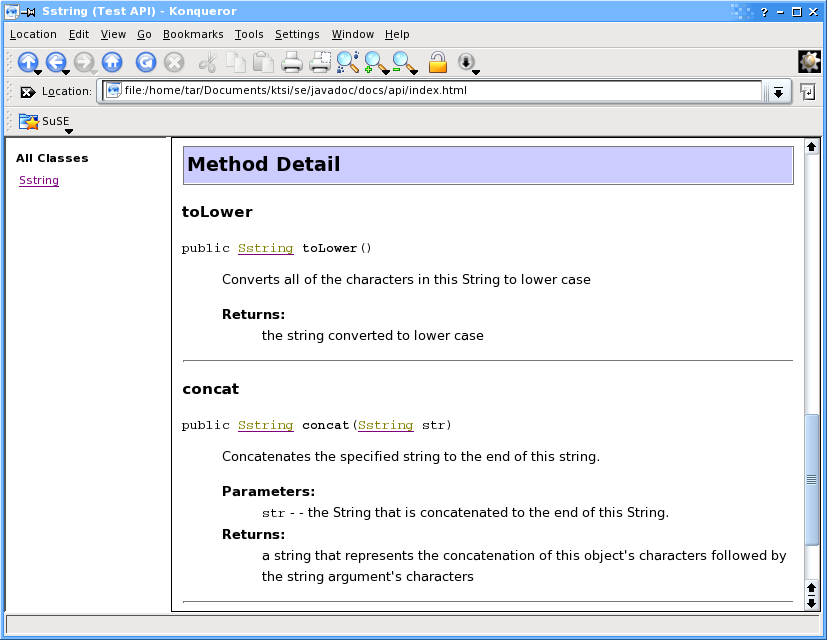
\includegraphics[width=0.6\linewidth]{qm/javadoc-example}
  \caption{Mit Javadoc erzeugte Dokumentation in HTML-Format}
  \label{fig:javadoc}
\end{figure}
%
\section{Further Informations}
\begin{itemize}
%\item Cem Kaner (Software Engineering, Florida Institute of Technology):
%    \href{http://www.kaner.com}{www.kaner.com}
\item Software Engineering Body of Knowledge:
  \href{http://www.swebok.org}{www.swebok.org}
\item Fit für Usability:
\href{http://www.fit-fuer-usability.de/archiv/category/usability_1x1/}
  {www.fit-fuer-usability.de/archiv/category/usability\_1x1}
\item Usability Forum:
\href{http://www.usability-forum.com/}{www.usability-forum.com/}
\end{itemize}
\section{Exercises}
\begin{enumerate}
\item Geben Sie für die Qualitätsmerkmale geeignete Masse/Messgrössen an, mit
  denen das betreffende Merkmal bewertet werden kann.
%\item
\end{enumerate}

%%% Local Variables:
%%% mode: latex
%%% TeX-master: "kurs"
%%% End:
